\documentclass{wissdoc}
% ----------------------------------------------------------------
% Abschlussarbeit - Hauptdokument
% ----------------------------------------------------------------
%%
%%
% wissdoc Optionen: draft, relaxed, pdf --> siehe wissdoc.cls
% ------------------------------------------------------------------
% Weitere packages: (Dokumentation dazu durch "latex <package>.dtx")
\usepackage[authoryear,sort&compress]{natbib}

\usepackage[utf8]{inputenc} % korrekte Darstellung von Umlauten
\usepackage[T1]{fontenc} % 字体编码支持
\usepackage{textcomp} % 文本符号支持
\usepackage[printonlyused]{acronym} % Abkürzungsverzeichnis nur mit Abkürzungen, die auch verwendet werden


% Reduce white space before chapter titles and remove "Kapitel" word
\usepackage{titlesec}
\titleformat{\chapter}[hang]
  {\normalfont\huge\bfseries}{\thechapter}{1em}{}
\titlespacing*{\chapter}{0pt}{0pt}{40pt}



% useful packages:
\usepackage{amsmath} % Standardpaket für Bereich Mathematik
\usepackage{amssymb} % zusätzliche Mathe-Symbole
\usepackage{tikz} % Diagramme und Skizzen
\usetikzlibrary{arrows.meta,positioning,calc}
% Captions: spacing, font, and justification
\usepackage{caption}
\usepackage{multirow}
\usepackage{svg}
\usepackage{graphicx}

% Below is the list of chapters
\captionsetup[figure]{skip=6pt,belowskip=8pt,justification=raggedright,singlelinecheck=false}
% Float spacing (space between text and floats)
\setlength{\textfloatsep}{12pt plus 3pt minus 3pt}
\setlength{\intextsep}{10pt plus 2pt minus 2pt}
\setlength{\floatsep}{12pt plus 3pt minus 3pt}
% \usepackage{rotating} % Rotation von z.B. Bildern, Tabellen etc.
% \usepackage{enumitem} % Kontrolle über Layout von itemize, enumerate, description
% \usepackage{pdfpages} % Seiten aus PDF/ ganzes PDF einbinden
% \usepackage{newunicodechar} % Bedeutung von Unicode Characters definieren, Nutzung über \newunicodechar{}{}


% \usepackage{varioref}
% \usepackage{verbatim}
% \usepackage{float}    %z.B. \floatstyle{ruled}\restylefloat{figure}
% \usepackage{subfigure}
% \usepackage{fancybox} % für schattierte,ovale Boxen etc.
% \usepackage{tabularx} % automatische Spaltenbreite
% \usepackage{supertab} % mehrseitige Tabellen
%% ---------------- end of usepackages -------------


%% Informationen für die PDF-Datei
\hypersetup{
 pdfauthor={N.N.},
 pdftitle={Not set},
 pdfsubject={Not set},
 pdfkeywords={Not set}
}

% Print URLs not in Typewriter Font
\def\UrlFont{\rm}

\newcommand{\blankpage}{% Leerseite ohne Seitennummer, nächste Seite rechts
 \clearpage{\pagestyle{empty}\cleardoublepage}
}

%% Einstellungen für das gesamte Dokument

% Trennhilfen
% Wichtig! 
% Im ngerman-paket sind zusätzlich folgende Trennhinweise enthalten:
% "- = zusätzliche Trennstelle
% "| = Vermeidung von Ligaturen und mögliche Trennung (bsp: Schaf"|fell)
% "~ = Bindestrich an dem keine Trennung erlaubt ist (bsp: bergauf und "~ab)
% "= = Bindestrich bei dem Worte vor und dahinter getrennt werden dürfen
% "" = Trennstelle ohne Erzeugung eines Trennstrichs (bsp: und/""oder)

% Trennhinweise fuer Woerter hier beschreiben
% \hyphenation{
% Pro-to-koll-in-stan-zen
% Ma-na-ge-ment  Netz-werk-ele-men-ten
% Netz-werk Netz-werk-re-ser-vie-rung
% Netz-werk-adap-ter Fein-ju-stier-ung
% Da-ten-strom-spe-zi-fi-ka-tion Pa-ket-rumpf
% Kon-troll-in-stanz
% }

% Index-Datei öffnen
\ifnotdraft{\makeindex}
%%%%%%%%%%%%%% includeonly %%%%%%%%%%%%%%%%%%%
% Es werden nur die Teile eingebunden, die hier 
% aufgefuehrt sind!
\includeonly{%
chapters/Abstract, % Abstract 
titelseite,%
erklaerung,% Declaration page
chapters/Introduction,% Chapter 1: Introduction
chapters/related_technologies,% Chapter 2: Related Technologies and Theoretical Foundations
chapters/hybrid_model,   % Chapter 3: Fault Diagnosis Model based on Hybrid Transformer-LSTM
chapters/experiments,      % Chapter 4: Experiments and Result Analysis
chapters/conclusion,  % Chapter 5: Conclusion and Future Work
anhang
}
%%%%%%%%%%%%%%%%%%%%%%%%%%%%%%%%%%%%%%%%%%%%%%
\begin{document}
\selectlanguage{english}

\renewcommand{\figurename}{Figure}
\renewcommand{\tablename}{Table}
\renewcommand{\bibname}{References}
\renewcommand{\chaptername}{Chapter}

\frontmatter
\pagenumbering{roman}
\ifnotdraft{
 %% Titelseite

\def\usesf{}
\let\usesf\sffamily % diese Zeile auskommentieren für normalen TeX Font

\newsavebox{\Erstgutachter}
\savebox{\Erstgutachter}{\usesf Prof.~Dr. Sax}
\newsavebox{\Zweitgutachter}
\savebox{\Zweitgutachter}{\usesf Prof.~Dr.}

\begin{titlepage}
\setlength{\unitlength}{1pt}
\begin{picture}(0,0)(85,770)

\includegraphics[width=\paperwidth]{logos/KIT_Deckblatt}
\end{picture}

%\vspace*{-39pt}\hspace*{300pt}
\includegraphics[width=.27\paperwidth]{logos/IOSB}
\vspace*{-39pt}\hspace*{300pt}
\includegraphics[width=.21\paperwidth]{logos/access_kit_rgb_logo.png}

\thispagestyle{empty}

%\begin{titlepage}
%%\let\footnotesize\small \let\footnoterule\relax
\begin{center}
\hbox{}
\vfill
{\usesf
{\huge\bfseries Hier steht der Titel der\\
                Diplom-/Studien-/Master-/""Bachelorarbeit \par}
\vskip 1.8cm
Diplomarbeit/Studienarbeit/Masterarbeit/Bachelorarbeit\\
von\\[2mm]
\vskip 1cm

{\large\bfseries Vorname Nachname\\}
\vskip 1.2cm
an der Fakultät für Informatik\\
Institut für Anthropomatik und Robotik\\
Zentrum für digitale Barrierefreiheit und Assistive Technologien (ACCESS@KIT)
\vskip 3cm
\begin{tabular}{p{5.5cm}l}
Erstgutachter: & \usebox{\Erstgutachter} \\
Zweitgutachter: & \usebox{\Zweitgutachter} \\
Betreuender~Mitarbeiter: &  M.Sc. \\
 & Dr. 
\end{tabular}
\vskip 3cm
Bearbeitungszeit:\qquad ??.~Monat~20?? -- ??.~Monat~20??
}
\end{center}
\vfill
\end{titlepage}
%% Titelseite Ende


%%% Local Variables: 
%%% mode: latex
%%% TeX-master: "thesis"
%%% End: 

 \blankpage % Leerseite auf Titelrückseite
 %
 % Die folgende Erklärung ist für Diplomarbeiten Pflicht
 % (siehe Prüfungsordnung), für Studienarbeiten nicht notwendig
 \thispagestyle{empty}
\vspace*{32\baselineskip}
\hbox to \textwidth{\hrulefill}
\par
I hereby declare that I have written this thesis independently and have not used any sources or aids other than those specified, that I have marked the passages taken literally or in terms of content as such, and that I have observed the statutes of the KIT for safeguarding good scientific practice in the currently valid version.

\vspace*{2cm}
Karlsruhe, den ??. ?????? 201?\hfill \hbox to 8cm{\hrulefill}

%%%%%%%%%%%%%%%%%%%%%%%%%%%%%%%%%%%%%%%%%%%%%%%%%%%%%%%%%%%%%%%%%%%%%%%%
%% Hinweis:
%%
%% Diese Erklärung wird von der Prüfungsordnung für Diplom-, Master,
%% und Bachelorarbeiten verlangt und ist zu unterschreiben. 
%% Für Studienarbeiten ist diese Erklärung nicht zwingend notwendig, 
%% schadet aber auch nicht.
%%%%%%%%%%%%%%%%%%%%%%%%%%%%%%%%%%%%%%%%%%%%%%%%%%%%%%%%%%%%%%%%%%%%%%%%
\clearpage







 \blankpage % Leerseite auf Erklärungsrückseite
}
%
%% *************** Hier geht's ab ****************
\chapter*{Abstract}

Industrial fault diagnosis represents a critical challenge in modern manufacturing systems, where early and accurate detection of equipment failures can prevent costly downtime and safety incidents. This thesis presents a novel hybrid Transformer-LSTM architecture for industrial fault diagnosis that combines the global attention mechanisms of Transformers with the sequential modeling capabilities of LSTM networks.

The proposed approach addresses the limitations of traditional fault diagnosis methods by effectively capturing both short-term fluctuations and long-term temporal dependencies in multi-dimensional industrial sensor data. The hybrid architecture employs a sophisticated feature fusion mechanism that leverages the complementary strengths of both neural network components while maintaining computational efficiency for real-time applications.

Extensive experimental evaluation on industrial datasets demonstrates the effectiveness of the proposed method, achieving 85.2\% classification accuracy across 11 different fault categories including backlash errors, bearing failures, and jerk motions. This performance significantly surpasses traditional approaches, with improvements of 6.9\% over pure LSTM networks, 3.5\% over pure Transformer architectures, and substantial gains over classical machine learning methods.

The system meets critical industrial requirements with an average inference time of 67ms per sample, enabling real-time fault detection and diagnosis. The modular design facilitates easy deployment and adaptation to different industrial environments and fault types.

This research contributes to the advancement of intelligent manufacturing systems and Industry 4.0 applications, providing a robust foundation for next-generation industrial fault diagnosis solutions. The hybrid approach opens new possibilities for combining different deep learning architectures to address complex temporal pattern recognition challenges in industrial automation.

%% ++++++++++++++++++++++++++++++++++++++++++
%% Verzeichnisse
%% ++++++++++++++++++++++++++++++++++++++++++
\setcounter{tocdepth}{2}
\ifnotdraft{
{\parskip 0pt\tableofcontents} % toc bitte einzeilig
\blankpage
\listoffigures
\blankpage
}


%% ++++++++++++++++++++++++++++++++++++++++++
%% Hauptteil
%% ++++++++++++++++++++++++++++++++++++++++++
\graphicspath{{Bilder/}}

\mainmatter
\pagenumbering{arabic}
\chapter{Introduction}
\label{cha:introduction}

\section{Research Background and Motivation}
\label{sec:introduction:background_motivation}

As industrial systems become more complex and automated under Industry 4.0, their reliability and safety are more critical than ever \cite{chen2017industry}. Unexpected equipment failures can lead to significant economic losses, production disruptions, and even safety accidents. Therefore, intelligent fault diagnosis technology, which can detect and identify potential faults in a timely and accurate manner, has become a key research area in industrial applications \cite{zhang2019deep, zhao2019deep}. Traditional fault diagnosis methods, which often rely on physical models or signal processing techniques combined with expert knowledge, struggle to cope with the massive, high-dimensional, and complex time-series data generated by modern sensor networks \cite{lei2016intelligent}. The data collected from industrial processes, such as vibration, pressure, and temperature signals, are often characterized by strong non-linearity and non-stationarity, making it difficult for these conventional methods to effectively extract discriminative fault features.

In recent years, data-driven approaches, particularly those based on deep learning, have shown great potential in overcoming these limitations \cite{liu2018artificial}. Deep learning models can automatically learn hierarchical features directly from raw sensor data, bypassing the need to manually design features, a process that is often slow and subjective \cite{khan2018review}. Among various deep learning architectures, Long Short-Term Memory (LSTM) networks, a specialized type of recurrent neural network (RNN), are particularly well-suited for modeling time-series data due to their ability to capture temporal dependencies \cite{hochreiter1997long}. LSTMs have been successfully applied to fault detection in industrial time series, demonstrating their effectiveness in learning from sequential patterns \cite{filonov2016multivariateindustrialtimeseries}. 

However, LSTMs process information sequentially, which can lead to challenges in capturing long-range dependencies in very long sequences and may suffer from computational inefficiency. More recently, the Transformer model, which relies entirely on a self-attention mechanism, has achieved state-of-the-art performance in various sequence modeling tasks \cite{vaswani2017attention}. The self-attention mechanism allows the Transformer to weigh the importance of all time steps simultaneously, enabling it to capture global dependencies and interactions within a sequence. This capability offers a new and powerful perspective for time-series analysis and has shown promise in fault diagnosis \cite{wen2021time}. Nevertheless, the standard Transformer architecture may not sufficiently capture the fine-grained, ordered nature of fault signatures as effectively as recurrent models.

This reveals a clear research gap: LSTMs excel at modeling local, sequential patterns but may miss critical long-range dependencies, while Transformers are adept at capturing global context but may overlook the nuanced, ordered progression inherent in fault evolution. The motivation for this thesis is that by combining the different strengths of these two architectures, it is possible to build a more effective model. This thesis hypothesizes that a hybrid model can achieve superior performance by leveraging the Transformer\'s ability to extract globally relevant features and then feeding these context-rich representations into an LSTM to model the temporal evolution of the system\'s health state. Furthermore, this research aims to address practical challenges such as class imbalance and multi-scale temporal patterns by proposing a novel hybrid Transformer-LSTM model that incorporates an adaptive fusion mechanism and a focal loss function, creating a fault diagnosis system that is both accurate and reliable.


\section{Analysis of Current Research Status}
\label{sec:introduction:current_status}

Fault diagnosis technology in the industrial sector has evolved through three main phases: physics-based models, traditional machine learning-based methods, and deep learning-based approaches \cite{lei2016intelligent, zhao2019deep}.

Early research primarily focused on physics-based models and signal processing techniques \cite{lei2020applications}. These methods attempt to build precise mathematical models for specific equipment or utilize techniques like Fourier Transform and Wavelet Transform to analyze signal characteristics in the time or frequency domain \cite{liu2018artificial}. However, these approaches often require extensive prior knowledge, involve complex model construction, and have limited generalization capabilities when faced with complex and variable operating conditions \cite{liu2018artificial}. Subsequently, traditional machine learning methods, represented by Support Vector Machines (SVM), k-Nearest Neighbors (k-NN), and Artificial Neural Networks (ANN), were introduced \cite{zhao2019deep}. While these methods improved the level of automation in diagnostics, their performance depended heavily on hand-crafted features. Designing these features is slow, difficult, and requires deep domain expertise, which prevented a fully automated diagnosis process \cite{lei2020applications, zhao2019deep}.

In recent years, data-driven methods, particularly those based on deep learning, have become the mainstream research direction in intelligent fault diagnosis due to their powerful capabilities in automatic feature extraction and non-linear modeling \cite{zhao2019deep, zhang2019deep, khan2018review}. Various deep learning models have been successfully applied \cite{lei2020applications, zhang2019deep}:

\begin{itemize}
    \item \textbf{Convolutional Neural Networks (CNN):} Initially achieving great success in image recognition, CNNs are now widely used to process one-dimensional signals like vibration and acoustic data, or their two-dimensional time-frequency representations \cite{zhang2019deep, liu2018artificial}. Through their unique convolutional and pooling operations, CNNs can effectively capture local correlations and translation-invariant features in signals, making them highly suitable for extracting discriminative fault patterns from industrial sensor data \cite{zhao2019deep, lei2020applications}.
    \item \textbf{Recurrent Neural Networks (RNN) and their variants:} RNNs, especially Long Short-Term Memory (LSTM) and Gated Recurrent Unit (GRU) networks, are specifically designed for processing sequential data \cite{hochreiter1997long}. They can effectively capture temporal dependencies, which is crucial for understanding the entire lifecycle of a fault from inception to evolution \cite{filonov2016multivariateindustrialtimeseries, khan2018review}. Nevertheless, these models may struggle to capture long-range dependencies in very long sequences due to issues like vanishing gradients \cite{pascanu2013difficulty}.
    \item \textbf{The Transformer Model:} To address the problem of long-range dependencies, the Transformer model, originally developed for natural language processing, was introduced to time-series analysis \cite{vaswani2017attention}. Its core self-attention mechanism allows for the parallel computation of dependencies between all elements in a sequence, enabling the direct capture of global information \cite{vaswani2017attention}. This has provided a new perspective for fault diagnosis, and studies have shown the great potential of Transformer-based models in time-series forecasting and classification tasks \cite{zhou2021informer, wen2021time}.
\end{itemize}

To combine the advantages of different models for superior performance, researchers have begun to explore hybrid deep learning models \cite{zhao2019deep, lei2020applications}. For instance, using a CNN to extract spatial features and then feeding the output to an LSTM for time-series modeling (CNN-LSTM) is a common and proven strategy \cite{khan2018review, zhao2019deep}. Similarly, attention mechanisms have been incorporated into traditional architectures to improve their ability to focus on relevant information \cite{bahdanau2015neural}. Recent studies have also explored the integration of different optimization techniques, such as adaptive learning rates \cite{kingma2014adam, loshchilov2019decoupled} and advanced regularization methods \cite{srivastava2014dropout}, to enhance model performance and robustness. The success of such combined models demonstrates that further improvements in diagnostic accuracy and robustness can be achieved by integrating the structural strengths of different architectures \cite{lei2020applications, khan2018review}. However, combining the Transformer's ability to see the "big picture" with the LSTM's skill in handling ordered sequences is still a new area of research. This gap presents a clear opportunity for the research in this thesis.




\section{Core Issues and Challenges}
\label{sec:introduction:issues_challenges}

Despite the progress in deep learning-based fault diagnosis, several core issues and challenges remain to be addressed to enhance the performance, robustness, and applicability of these models in real-world industrial settings. This thesis will focus on the following key challenges:

\subsection{Modeling of Long-Term Time-Dependent Relationships}
Industrial processes often exhibit complex temporal dynamics where the signature of a fault may evolve over a long period. Capturing these long-range dependencies is crucial for early and accurate diagnosis. While LSTMs are designed to model temporal sequences, they can struggle with very long sequences due to the risk of vanishing or exploding gradients \cite{pascanu2013difficulty}, making it difficult to relate current observations to events far in the past. The challenge lies in developing a model that can effectively bridge these long time lags and understand the complete temporal evolution of system behavior.

\subsection{Data Class Imbalance}
In real-world industrial applications, datasets for fault diagnosis are often highly imbalanced. Data for normal operating conditions are abundant, while data for specific fault types, especially critical or catastrophic failures, are scarce. This imbalance can severely bias a machine learning model, causing it to perform well on the majority class (normal operation) but poorly on the minority classes (faults). The challenge is to design a model and training strategy that can learn effectively from imbalanced data, for instance by using specialized sampling techniques \cite{chawla2002smote}, and accurately identify rare but critical fault events.

\subsection{Multi-Scale Time Pattern Analysis}
Fault signatures in time-series data can manifest at multiple time scales. For example, a gradual degradation process might be a long-term trend, while an intermittent fault could appear as a short-term, high-frequency burst. A robust diagnostic system must be capable of simultaneously analyzing and integrating information from these different time scales. Traditional models often focus on a single temporal resolution, potentially missing important patterns at other scales. The challenge is to develop an architecture that can effectively extract and fuse multi-scale temporal features \cite{zhang2019deep} to form a comprehensive understanding of the system's health state.

\begin{figure}[h!]
\centering
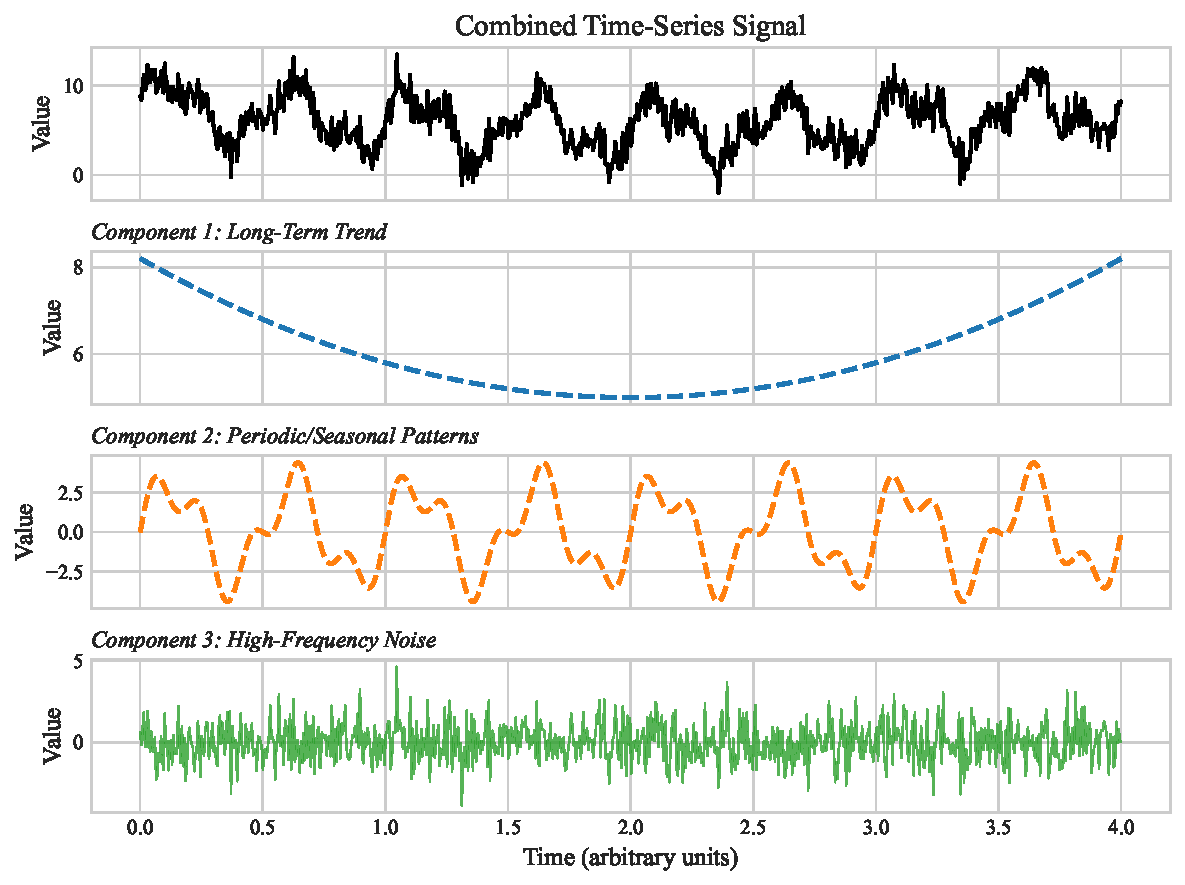
\includegraphics[width=0.8\textwidth]{logos/multi_scale_timeseries_decomposition.pdf}
\caption{An illustration of a complex time-series signal decomposed into its multi-scale components: a long-term trend, periodic patterns, and high-frequency noise.}
\label{fig:multi_scale_decomposition}
\end{figure}

\subsection{Generalization Ability to Different Working Conditions}
Industrial equipment often operates under various working conditions, such as different loads, speeds, or environmental factors. A fault diagnosis model trained on data from one set of conditions may not generalize well to others, as the fault signatures can vary significantly. This lack of generalization, often addressed with transfer learning techniques \cite{lei2020applications}, limits the practical deployment of diagnostic systems. The challenge is to build a model that is robust to variations in operating conditions and can extract invariant fault features, ensuring reliable performance across the full operational spectrum of the machinery.

\section{Main Research Content and Contributions}
\label{sec:introduction:content_contributions}

To address the challenges in industrial fault diagnosis, this thesis develops and tests a new hybrid deep learning system. The primary research content of this work is centered around building a hybrid architecture that combines Transformer and Long Short-Term Memory (LSTM) networks for better diagnostic performance. The key tasks undertaken in this research include:

Designing a Hybrid Transformer-LSTM Architecture: The main goal is to build a model that uses the unique strengths of both its parts. A Transformer encoder is employed to capture global dependencies and long-range correlations from multivariate sensor data, while a subsequent bidirectional LSTM (Bi-LSTM) network models the temporal evolution and sequential nature of the extracted features.

Developing an Adaptive Feature Fusion Strategy: A key part of the hybrid model is how it combines features from the Transformer and LSTM. This research proposes an adaptive fusion method that intelligently blends global context from the Transformer with local temporal patterns from the LSTM, helping the model focus on the most important information for diagnosis.

Addressing Real-World Challenges: This study also tackles practical issues commonly found in industrial environments, beyond just the core architecture. This includes utilizing a focal loss function to mitigate the effects of class imbalance, applying targeted data augmentation techniques for time-series data, and ensuring the model's robustness through appropriate regularization and training strategies.

Experimental Validation: The proposed model is thoroughly tested on a real industrial dataset with various fault types (e.g., backlash, baseline shift, jerk). Performance is compared against baseline models, including standalone Transformer and LSTM architectures, using detailed experiments and ablation studies.

The main contributions of this thesis, both theoretical and practical, are summarized as follows:

A New Hybrid Deep Learning Architecture for Fault Diagnosis: This thesis introduces a new hybrid model that successfully integrates Transformer and LSTM networks. This architecture offers a new way to analyze industrial time-series data. It models both global feature interactions and local temporal dynamics at the same time, overcoming a major limitation of using either model alone \cite{wen2021time}.

An Adaptive Fusion Mechanism for Better Feature Representation: This thesis proposes an adaptive fusion strategy that effectively combines features from different levels. Unlike simple concatenation, this mechanism allows the model to learn the optimal balance between global and sequential representations, leading to a more robust and discriminative feature space for classification.

A Complete Solution to Common Industrial Data Challenges: This research offers a comprehensive approach that tackles several practical problems at once. By integrating techniques like focal loss for class imbalance \cite{lin2017focal} and advanced regularization, this work provides a more complete and robust solution for real industrial applications.

Experimental Results and Practical Guidance for Industry: Through extensive experiments, this thesis shows that the proposed model performs better than conventional and single-architecture deep learning methods. The detailed methods and positive results offer practical guidance for implementing advanced AI-driven predictive maintenance systems in industrial settings.

\section{Thesis Chapter Organization}
\label{sec:introduction:organization}

The remainder of this thesis is structured as follows:

Chapter 2: Related Technologies and Theoretical Foundations provides a comprehensive review of the fundamental concepts underpinning this research. It covers the principles of Long Short-Term Memory (LSTM) networks, the architecture of the Transformer model, including the self-attention mechanism, and other key deep learning techniques relevant to this study.

Chapter 3: Fault Diagnosis Model based on Hybrid Transformer-LSTM details the proposed model. It presents the overall architecture, describes the data preprocessing pipeline, and elaborates on the design of the Transformer feature extraction component, the LSTM sequence modeling component, and the core adaptive feature fusion strategy.

Chapter 4: Experiments and Result Analysis describes the experimental setup, including the dataset, evaluation metrics, and hyperparameter settings. It presents a detailed analysis of the experimental results, including performance comparisons with baseline models, ablation studies to validate the contribution of each model component, and visualizations such as confusion matrices and learning curves.

Chapter 5: Conclusion and Future Work summarizes the key findings and and contributions of this research. It also discusses the limitations of the current work and suggests potential directions for future research, such as model optimization for real-time deployment and exploration of unsupervised learning methods.  % Chapter 1: Introduction
\chapter{Related Technologies and Theoretical Foundations}
\label{cha:related_technologies}

This chapter provides a comprehensive review of the fundamental technologies and theoretical foundations underlying the proposed hybrid Transformer-LSTM model. The chapter is organized into two main sections that examine the core architectures essential to this research. First, we explore Long Short-Term Memory (LSTM) networks, discussing their gating mechanisms, bidirectional capabilities, and their effectiveness in capturing sequential dependencies in time-series data. Second, we examine the Transformer architecture, focusing on its self-attention mechanism, multi-head attention, and encoder structure that enables parallel processing and global context modeling. Together, these technologies form the theoretical foundation for understanding how their complementary strengths can be combined to create a more robust fault diagnosis system.

\section{Long Short-Term Memory Networks (LSTM)}
\label{sec:related_technologies:lstm}

This section reviews recurrent neural networks (RNNs) and the challenges of training them, introduces the Long Short-Term Memory (LSTM) architecture and its gating mechanism, discusses the strengths and limitations of LSTMs for time-series modeling, and explains the principle of Bidirectional LSTM (Bi-LSTM).

\subsection{RNN Basics and the Vanishing/Exploding\\ Gradient Problem}
An RNN processes a sequence \(\mathbf{x}_t\) by maintaining a hidden state \(\mathbf{h}_t\) that is updated recurrently as:
\begin{equation}
\mathbf{h}_t = \phi(\mathbf{W}_{xh}\,\mathbf{x}_t + \mathbf{W}_{hh}\,\mathbf{h}_{t-1} + \mathbf{b}_h)
\label{eq:rnn_update}
\end{equation}
where \(\phi\) is a nonlinearity. Training is typically done via backpropagation through time (BPTT), which unrolls the network over temporal steps. In long sequences, repeated multiplication by Jacobians leads to gradients that either shrink towards zero (vanish) or grow uncontrollably (explode), hampering the learning of long-range dependencies and causing optimization instability \cite{pascanu2013difficulty}. Gradient clipping mitigates exploding gradients, but vanishing gradients remain a central obstacle for standard RNNs to capture dependencies spanning many time steps.

More concretely, the gradient across \(k\) steps contains products like:
\begin{equation}
\prod_{i=1}^{k} \frac{\partial \mathbf{h}_{t-i+1}}{\partial \mathbf{h}_{t-i}}
\label{eq:gradient_product}
\end{equation}
When the spectral radius of the recurrent Jacobian is smaller (greater) than one on average, gradients decay (blow up) exponentially with \(k\), which explains why plain RNNs struggle with long-term credit assignment. Practical workarounds include truncated BPTT (limiting the backpropagated horizon), gradient clipping for stability, careful initialization (e.g., orthogonal \(\mathbf{W}_{hh}\)), and using gates or skip/residual connections to create more favorable gradient pathways \cite{pascanu2013difficulty}. These heuristics help but do not fully resolve vanishing gradients in vanilla RNNs, which motivates gated architectures such as the LSTM.

From a training perspective, backpropagation through time over a window of length \(K\) costs roughly:
\begin{equation}
\mathcal{O}(K \cdot (d_x d_h + d_h^2))
\label{eq:bptt_complexity}
\end{equation}
per sequence, where \(d_x\) and \(d_h\) are the input and hidden dimensions. Truncated BPTT chooses a moderate \(K\) (e.g., 50--200 steps) to balance long-range learning with computational and memory budgets. Gradient clipping commonly constrains the global norm:
\begin{equation}
\lVert \nabla \rVert_2 \leftarrow \min(\lVert \nabla \rVert_2, \tau)
\label{eq:gradient_clipping}
\end{equation}
to avoid instability when occasional large Jacobian products arise.

Finally, activation choices matter: saturating nonlinearities (sigmoid, tanh) have derivatives bounded by \((0, 0.25]\) and \((0, 1]\) respectively, which can compound vanishing; non-saturating alternatives (ReLU) improve gradient flow but complicate recurrent stability and may cause unbounded activations without care. These trade-offs further motivate gated RNNs that provide an explicit additive path for gradients.

\subsection{LSTM Gates and Working Mechanism}

LSTM networks address vanishing gradients by introducing an additive memory pathway---the cell state \(\mathbf{c}_t\)---and multiplicative gates that regulate information flow \cite{hochreiter1997long}. 

\paragraph{Core LSTM Equations.} At each time step, the LSTM computes the following gates and states:
\begin{align}
\mathbf{f}_t &= \sigma(\mathbf{W}_f [\mathbf{x}_t, \mathbf{h}_{t-1}] + \mathbf{b}_f) &&\text{(forget gate)}\\
\mathbf{i}_t &= \sigma(\mathbf{W}_i [\mathbf{x}_t, \mathbf{h}_{t-1}] + \mathbf{b}_i) &&\text{(input gate)}\\
\tilde{\mathbf{c}}_t &= \tanh(\mathbf{W}_c [\mathbf{x}_t, \mathbf{h}_{t-1}] + \mathbf{b}_c) &&\text{(candidate state)}\\
\mathbf{c}_t &= \mathbf{f}_t \odot \mathbf{c}_{t-1} + \mathbf{i}_t \odot \tilde{\mathbf{c}}_t &&\text{(cell update)}\\
\mathbf{o}_t &= \sigma(\mathbf{W}_o [\mathbf{x}_t, \mathbf{h}_{t-1}] + \mathbf{b}_o) &&\text{(output gate)}\\
\mathbf{h}_t &= \mathbf{o}_t \odot \tanh(\mathbf{c}_t) &&\text{(hidden state)}
\end{align}

where \(\sigma\) denotes the logistic sigmoid function and \(\odot\) represents element-wise multiplication.

\paragraph{Key Innovation: Additive Cell State.} The critical innovation lies in the cell-state update equation \(\mathbf{c}_t = \mathbf{f}_t \odot \mathbf{c}_{t-1} + \mathbf{i}_t \odot \tilde{\mathbf{c}}_t\), which preserves information through additive interactions modulated by gates. This creates a constant error carousel that supports more stable gradient flow across time. Unlike vanilla RNNs that suffer from repeated matrix multiplications during backpropagation, this additive update mechanism provides an almost unattenuated pathway for gradients, enabling LSTMs to learn both short- and moderately long-range temporal dependencies \cite{hochreiter1997long}.

\paragraph{Gate Functions and Information Flow.} As illustrated in Figure~\ref{fig:lstm_cell_diagram}, each gate serves a specific purpose:
\begin{itemize}
    \item \textbf{Forget gate} \(\mathbf{f}_t\): Controls what information to discard from the cell state
    \item \textbf{Input gate} \(\mathbf{i}_t\): Determines which values to update in the cell state
    \item \textbf{Candidate state} \(\tilde{\mathbf{c}}_t\): Generates new candidate values to be added
    \item \textbf{Output gate} \(\mathbf{o}_t\): Controls which parts of the cell state to output
\end{itemize}

The gates jointly regulate how information is retained, written, and exposed from the cell state, providing a practical implementation of the mathematical formulations above.

% External figure referenced above
\begin{figure}[tbp]
\centering
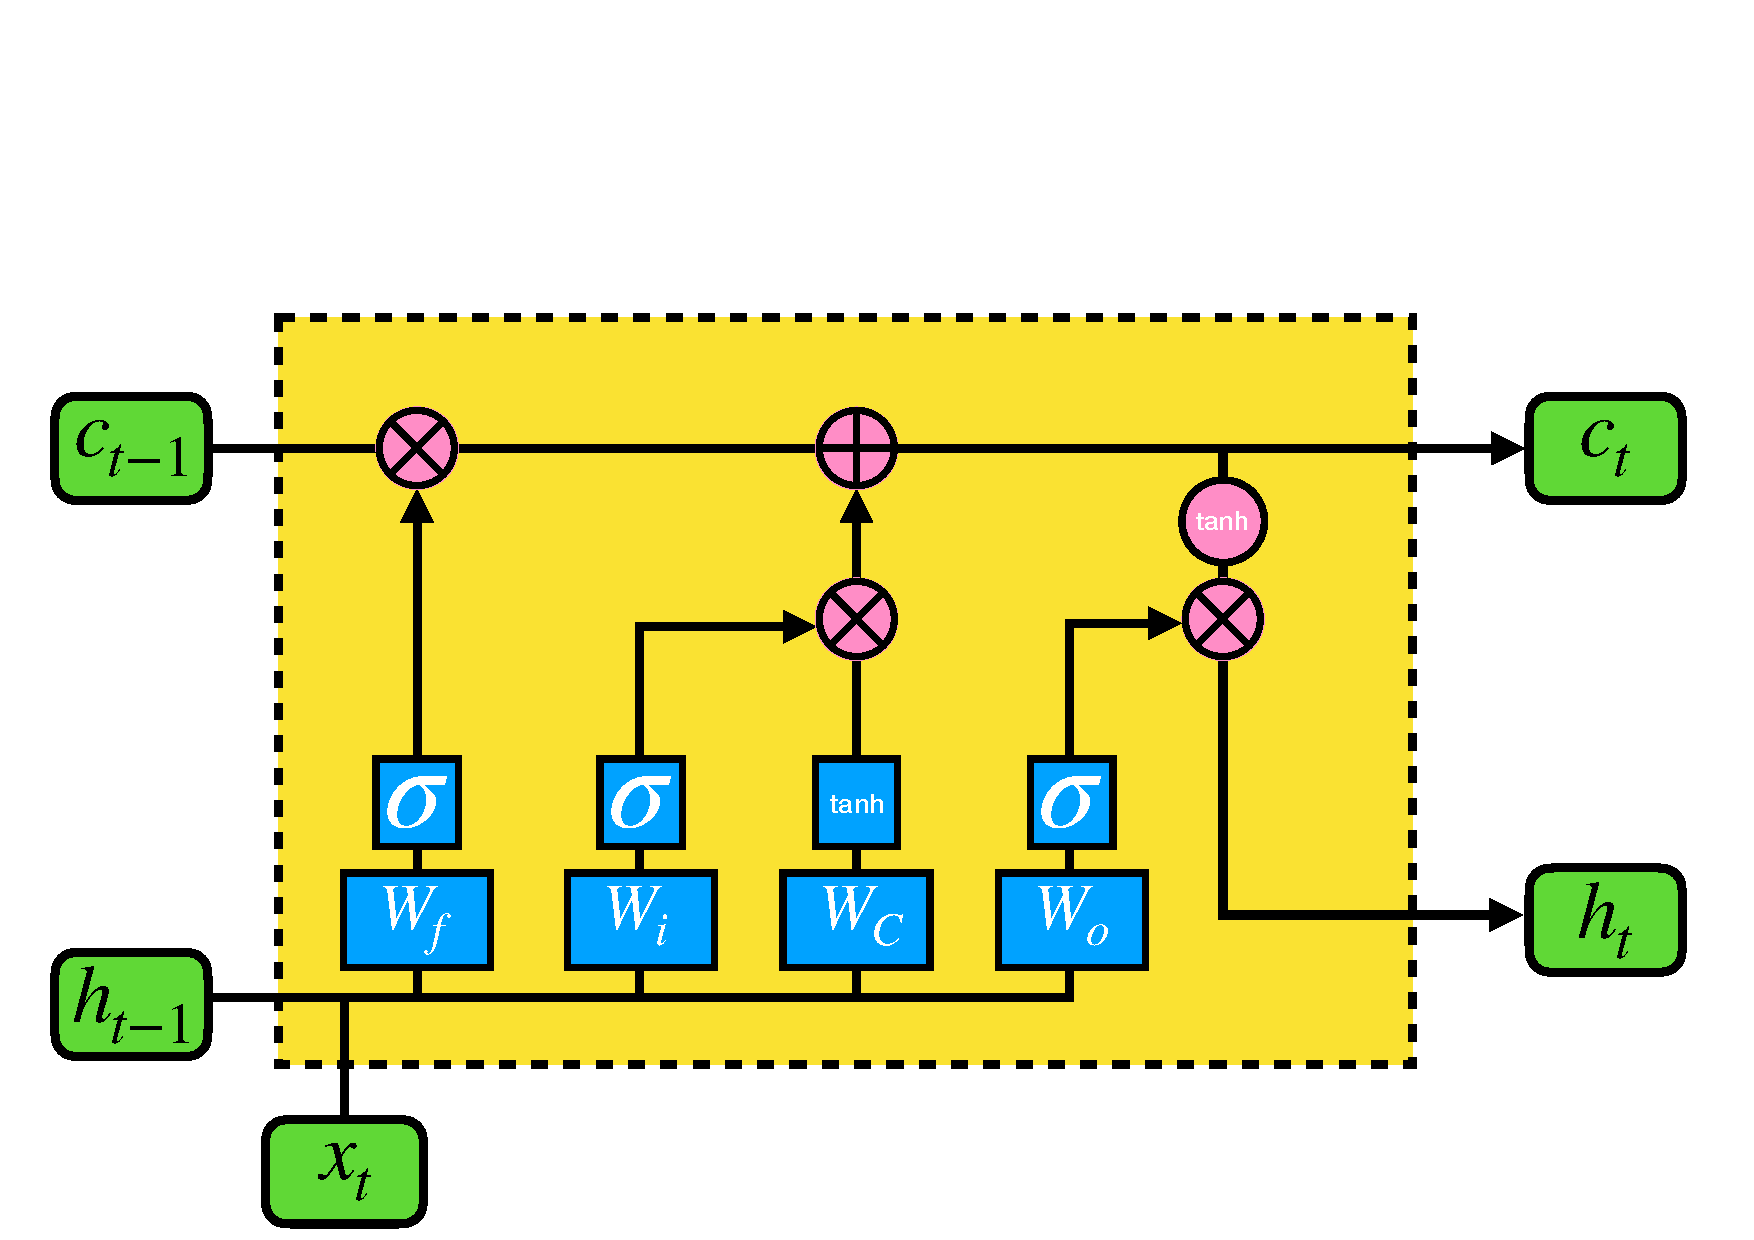
\includegraphics[width=0.7\textwidth]{logos/ClassicalLSTM_Diagram.pdf}
\caption[LSTM cell diagram]{A schematic diagram of the classical long short-term memory (LSTM) cell architecture, showing the three gates (forget, input, output) and the cell state pathway. \cite{chen2020quantumlongshorttermmemory}}
\label{fig:lstm_cell_diagram}
\end{figure}

\paragraph{Common Variants and Extensions.} Beyond the basic cell, common variants add peephole connections (letting gates observe \(\mathbf{c}_{t-1}\)/\(\mathbf{c}_t\)), or initialize the forget gate bias positively to encourage longer retention at the start of training. Intuitively, the partial derivative \(\partial \mathbf{c}_t/\partial \mathbf{c}_{t-1} = \mathbf{f}_t\) explains how the forget gate directly scales gradient flow along the cell state pathway; values of \(\mathbf{f}_t\) near one help preserve information and gradients over time.

\paragraph{Computational Cost and Practical Considerations.} If \(\mathbf{x}_t \in \mathbb{R}^{d_x}\), \(\mathbf{h}_t, \mathbf{c}_t \in \mathbb{R}^{d_h}\), each gate uses an affine map with parameters of size \(d_h\times(d_x+d_h)\) plus bias. Four such maps imply a per-step cost of order \(\mathcal{O}(d_h(d_x+d_h))\) and memory proportional to activations over time. In practice, mini-batch computation dominates wall time; masking or packed sequences prevent padded timesteps from contributing spurious gradients.

\paragraph{Gate Saturation Regimes.} When \(\mathbf{f}_t\) saturates near 1 while \(\mathbf{i}_t \approx 0\), the LSTM behaves as a leaky integrator that retains past information; conversely, \(\mathbf{f}_t\) near 0 forgets rapidly. The output gate \(\mathbf{o}_t\) modulates exposure of the internal memory to downstream layers; throttling \(\mathbf{o}_t\) can stabilize training early on at the cost of slower information throughput.

\paragraph{Advanced Training Techniques.} Normalization inside the cell (e.g., layer normalization on gate pre-activations) can reduce covariate shift across time and ease optimization, sometimes enabling larger learning rates. Coupled input–forget gate (CIFG) variants tie \(\mathbf{f}_t = 1-\mathbf{i}_t\) to reduce parameters and encourage complementary behavior; while parameter-efficient, CIFG may be less expressive on tasks requiring independent retention and write controls. Peepholes let gates read the cell state and can improve precise temporal counting.

\paragraph{A short gradient derivation.} By unrolling the cell-state update, one obtains
\begin{align}
\frac{\partial \mathbf{c}_t}{\partial \mathbf{c}_{t-1}} &= \mathbf{f}_t,\quad\; \frac{\partial \mathbf{c}_{t-1}}{\partial \mathbf{c}_{t-2}} = \mathbf{f}_{t-1},\; \ldots \\
\Rightarrow\; \frac{\partial \mathbf{c}_t}{\partial \mathbf{c}_{t-k}} &= \prod_{j=t-k+1}^{t} \mathbf{f}_j.
\end{align}
When the forget gates are near one, this multiplicative path preserves gradients over long spans; when they are small, information is intentionally forgotten.

\paragraph{LSTM forward steps (per time \(t\)).} Given \(\mathbf{x}_t\) and \((\mathbf{h}_{t-1},\mathbf{c}_{t-1})\): (1) compute gates \(\mathbf{f}_t,\mathbf{i}_t,\mathbf{o}_t\) and candidate \(\tilde{\mathbf{c}}_t\); (2) update memory \(\mathbf{c}_t = \mathbf{f}_t\odot\mathbf{c}_{t-1}+\mathbf{i}_t\odot\tilde{\mathbf{c}}_t\); (3) expose state \(\mathbf{h}_t = \mathbf{o}_t\odot \tanh(\mathbf{c}_t)\). Mini-batch masking ensures padded steps neither affect gate activations nor the loss.

\subsection{LSTM Variants and Training Techniques}
Beyond the vanilla cell, a number of practical variants and training techniques are widely adopted to improve optimization stability and efficiency:
\begin{itemize}
    \item \textbf{Peephole connections} let gates access the cell state \(\mathbf{c}_{t-1}\) or \(\mathbf{c}_t\) directly, tightening control over precise counting and timing \citep{gers2000learning}. This variant has shown improvements in tasks requiring precise temporal modeling.
    \item \textbf{Coupled input–forget gate (CIFG)} ties \(\mathbf{f}_t = 1-\mathbf{i}_t\) to reduce parameters and encourage complementary behavior; while parameter-efficient, decoupled gates can be more expressive when retention and writing need to be controlled independently \citep{greff2017lstm}.
    \item \textbf{Normalization in RNNs} (e.g., layer normalization applied to gate pre-activations) reduces internal covariate shift and can enable larger learning rates and deeper stacks \citep{ba2016layer}. Recent work has shown significant improvements in training stability and convergence speed.
    \item \textbf{Recurrent dropout/Zoneout}. Instead of dropping inputs only, apply structured noise on recurrent connections or randomly preserve previous hidden states to regularize temporal dynamics while keeping information flow stable \citep{krueger2017zoneout, semeniuta2016recurrent}.
    \item \textbf{Initialization and clipping}. Orthogonal initialization of \(\mathbf{W}_{hh}\), positive bias for forget gates, and global-norm gradient clipping (e.g., 0.5--5.0) are common to mitigate exploding gradients \citep{pascanu2013difficulty, jozefowicz2015empirical}.
    \item \textbf{Packing/masking}. For variable-length sequences, use padding masks (or packed sequences) to prevent padded steps from contributing to attention, gates, or the loss \citep{goodfellow2016deep}.
\end{itemize}
Stacking 2--3 LSTM layers with residual or skip connections often improves representation power with modest overhead \citep{he2016deep}. In industrial time-series, stacking is typically combined with temporal pooling or attention to summarize features for classification \citep{zhao2019deep}.

\subsection{Strengths and Limitations for Time-Series Modeling}
\textbf{Strengths.} LSTMs are effective at modeling sequential dependencies, handling variable-length inputs, and integrating multivariate sensor streams. Their gating mechanism helps filter noise and retain salient temporal patterns, which has led to strong results in industrial time-series fault detection and prediction \cite{filonov2016multivariateindustrialtimeseries, zhao2019deep}. They naturally support many-to-one (sequence classification), many-to-many (sequence labeling), and sequence-to-sequence settings. In practice, padding and masking let LSTMs consume mini-batches of variable-length sequences without corrupting gradients. When paired with dropout/Zoneout and early stopping, LSTMs generalize well on moderately sized datasets.

\textbf{Limitations.} Despite improved gradient flow, LSTMs can still struggle with very long sequences and long-range interactions spanning hundreds or thousands of steps. Their inherently sequential computation limits parallelism on modern accelerators, yielding higher training latency and memory usage compared with attention-based models. Performance can be sensitive to depth, hidden size, and regularization choices; small datasets may overfit without proper constraints. Moreover, when global context is crucial, attention-based architectures such as the Transformer can capture long-range dependencies more efficiently via direct pairwise interactions and highly parallel computation \cite{pascanu2013difficulty, vaswani2017attention}. In forecasting, encoder-decoder hybrids (e.g., LSTM encoder with attention) are often adopted to mitigate these limitations.

\textbf{Implementation notes.} Normalization (z-score per channel), careful learning-rate schedules (e.g., cosine decay with warmup), and gradient clipping thresholds tuned between 0.5 and 5.0 are common. For class-imbalanced fault data, weighted losses or focal loss can complement LSTM modeling; early anomaly detection may benefit from shorter truncation windows updated more frequently, whereas long-horizon forecasting uses longer windows at the expense of compute.

\textbf{Data windowing and leakage.} For supervised time-series learning, choose window length and stride to reflect the process dynamics (e.g., at least a few dominant periods of vibration). Ensure no temporal leakage from future segments into training windows for validation/test splits; use contiguous block splits when distribution shift over time is plausible. Missing values can be handled with masking inputs and, optionally, time-since-last-observation channels to inform the model about gaps.

\begin{table}[t]
\centering
\caption{Typical LSTM configuration choices (indicative ranges; tune on validation).}
\label{tab:lstm_config}
\begin{tabular}{l l}
\hline
Hidden size \(d_h\) & 64--256, increase with data size/complexity \\
Layers & 1--3 (stacked), residual skip if \(\geq 3\) \\
Dropout & 0.1--0.5 between layers (avoid inside gates) \\
Truncated BPTT \(K\) & 50--200 steps depending on context length \\
Clip norm & 0.5--5.0 (global \(\ell_2\)) \\
LR & \(10^{-3}\) to \(10^{-4}\) with Adam/decoupled weight decay \\
Batching & Pad + mask or packed sequences to handle variable length \\
\hline
\end{tabular}
\end{table}

\begin{table}[t]
\centering
\caption{Qualitative comparison of sequence models for industrial time-series.}
\label{tab:model_compare}
\begin{tabular}{p{2.8cm} p{3.2cm} p{3.2cm} p{3.8cm}}
\hline
\textbf{Aspect} & \textbf{LSTM} & \textbf{GRU} & \textbf{Transformer} \\
\hline
Parameters & Higher (4 gates) & Lower (3 gates) & High (attention blocks) \\[0.5ex]
Parallelism & Low (sequential) & Low (sequential) & High (token-parallel) \\[0.5ex]
Long-range dependencies & Moderate (via gates) & Moderate & Strong with attention \\[0.5ex]
Latency (causal) & Good (uni-directional) & Good (uni-directional) & Moderate (causal masks) \\[0.5ex]
Data requirements & Moderate & Moderate & Higher for stability \\
\hline
\end{tabular}
\end{table}

\subsection{Bidirectional LSTM (Bi-LSTM)}
Bi-LSTM extends the standard LSTM by running two LSTMs in parallel: one processes the sequence forward (from \(t=1\) to \(T\)) and the other backward (from \(t=T\) to \(1\)). The two hidden representations are then concatenated (or combined) to form a context-enriched feature at each time step. This provides the model with information from both past and future contexts, which often improves performance on sequence classification and labeling tasks where the full sequence is available at inference time. However, Bi-LSTM is not causal and thus unsuitable for strict real-time scenarios that cannot access future observations. In machinery health monitoring and fault diagnosis, Bi-LSTMs have been widely adopted as a strong baseline due to their enhanced context modeling capability \cite{zhang2019deep, zhao2019deep}.

\begin{figure}[!h]
\centering
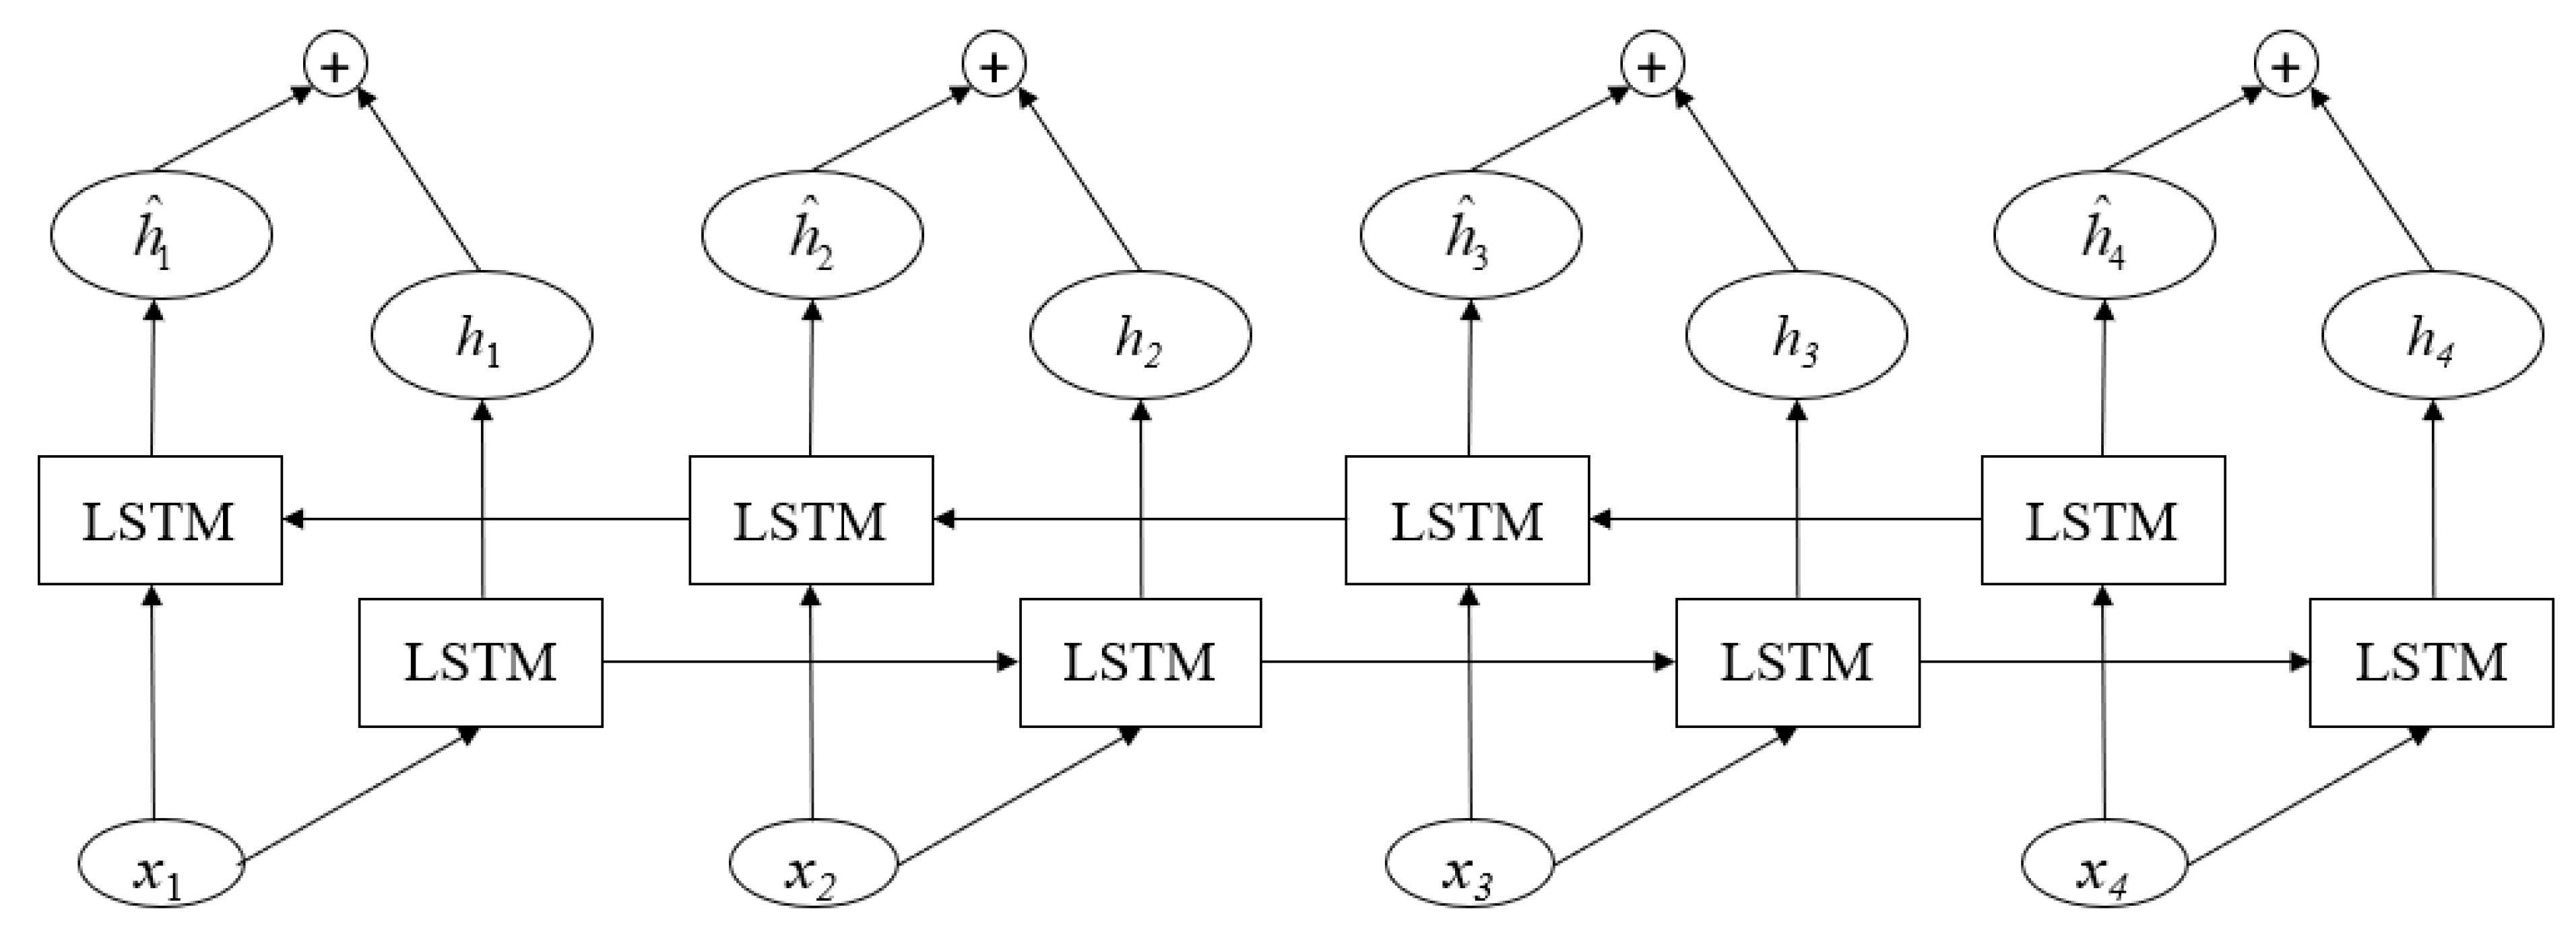
\includegraphics[width=0.8\textwidth]{logos/BI-LSTM.png}
\caption[Bidirectional LSTM architecture]{A schematic diagram of the bidirectional LSTM (Bi-LSTM) architecture\cite{s21206758}}
\end{figure}

In practice, Bi-LSTMs are commonly followed by temporal pooling (e.g., max/mean over time) or attention layers to summarize step-wise representations into a fixed-size vector for downstream classification. The bidirectional setup increases parameters and compute compared to a single-direction LSTM, so batch size and sequence length may need tuning to fit memory constraints. For causal or low-latency systems, a uni-directional LSTM (or streaming variants) is preferred.

Formally, if the forward and backward hidden states at step \(t\) are \(\overrightarrow{\mathbf{h}}_t\) and \(\overleftarrow{\mathbf{h}}_t\), a common fusion is concatenation \(\mathbf{z}_t = [\overrightarrow{\mathbf{h}}_t;\,\overleftarrow{\mathbf{h}}_t]\) followed by a classifier \(\mathbf{y}_t = g(\mathbf{W}\mathbf{z}_t + \mathbf{b})\). Pooling over \(t\) or selecting the last step yields sequence-level predictions. Memory and compute roughly double versus a single-direction LSTM with the same \(d_h\).
\par
Where strict causality is not required but low latency matters, limited look-ahead (e.g., a few timesteps) can approximate bidirectional context in streaming by buffering short chunks. For structured sequence labeling (e.g., event boundary detection), a Bi-LSTM encoder paired with a CRF decoding layer can enforce label consistency over time; in classification, simple temporal pooling often suffices.

Conceptually, a Bi-LSTM processes each input step with a forward and a backward LSTM; their hidden states are concatenated and passed to a classifier or pooling layer.


\section{Transformer Model}
\label{sec:related_technologies:transformer}

The Transformer, introduced by \cite{vaswani2017attention}, represents a paradigm shift in sequence modeling, moving away from recurrent architectures and embracing self-attention as its core mechanism. This allows for significantly more parallelization and has established new standards in natural language processing and beyond \citep{zhou2021informer, zhao2019deep}. This section details the foundational concepts of the Transformer, including the attention mechanism, its multi-head variant, and the overall architecture of the encoder block.

\subsection{The Basic Idea of the Attention Mechanism}
The attention mechanism was developed to address the limitations of fixed-length context vectors in traditional encoder-decoder models, where the decoder had to rely on a single vector summarizing the entire input sequence. Attention provides a solution by allowing the model to dynamically focus on different parts of the input sequence when producing an output at a specific time step.

The core idea is to compute a set of attention weights for each element in the input sequence. These weights determine the importance of each input element relative to the current output position. The final output is then a weighted sum of the input representations, where the weights are the computed attention scores. This mechanism enables the model to selectively draw upon the most relevant information from the input, regardless of its position, thereby improving its ability to handle long-range dependencies.
Classical formulations of attention in encoder–decoder models trace back to \cite{bahdanau2015neural}, while modern scaled dot-product attention popularized by \cite{vaswani2017attention} enables highly parallel computation.

\subsection{The Calculation Process of the Self-Attention Mechanism}
Self-attention, also known as intra-attention, is a specific type of attention mechanism that allows a model to weigh the importance of different words within the same sequence. Instead of relating an input and an output sequence, it relates different positions of a single sequence to compute a representation of that sequence.

The calculation is based on three vectors derived from each input embedding: the Query (\(\mathbf{Q}\)), the Key (\(\mathbf{K}\)), and the Value (\(\mathbf{V}\)). These vectors are generated by multiplying the input embedding by three distinct weight matrices.
The process can be summarized in three steps:
\begin{enumerate}
    \item \textbf{Compute Scores:} The score for each position is calculated by taking the dot product of the Query vector of the current position with the Key vectors of all positions in the sequence. This determines how much attention the current position should pay to every other position.
    \item \textbf{Scale and Normalize:} The scores are scaled down by dividing by the square root of the dimension of the key vectors, \(\sqrt{d_k}\). This scaling prevents the dot products from growing too large and pushing the softmax function into regions with very small gradients. A softmax function is then applied to the scaled scores to obtain the attention weights, which are positive and sum to one.
    \item \textbf{Compute Output:} The final output for the position is a weighted sum of the Value vectors, where the weights are the normalized attention scores from the previous step.
\end{enumerate}
This entire computation is captured compactly in the following equation:
\begin{equation}
    \text{Attention}(\mathbf{Q}, \mathbf{K}, \mathbf{V}) = \text{softmax}\left(\frac{\mathbf{Q}\mathbf{K}^T}{\sqrt{d_k}}\right)\mathbf{V}
    \label{eq:self_attention}
\end{equation}

\subsection{The Advantages of Multi-Head Attention}
A single self-attention mechanism can be limiting, as it only allows the model to focus on other positions in one way. The Transformer enhances this by introducing Multi-Head Attention. Instead of performing a single attention function, this mechanism runs multiple attention calculations in parallel.

The primary advantages of this approach are:
\begin{itemize}
    \item \textbf{Diverse Representations:} Each "head" uses different, learned linear projections to transform the input Queries, Keys, and Values. This allows each head to learn to attend to different types of relationships or information from different representation subspaces. For example, one head might learn to capture syntactic relationships, while another focuses on semantic ones.
    \item \textbf{Enriched Feature Combination:} The outputs of all the parallel attention heads are concatenated and passed through a final linear projection. This allows the model to combine the various learned relationships into a single, richer representation for each position.
\end{itemize}

\begin{figure}[htb]
\centering
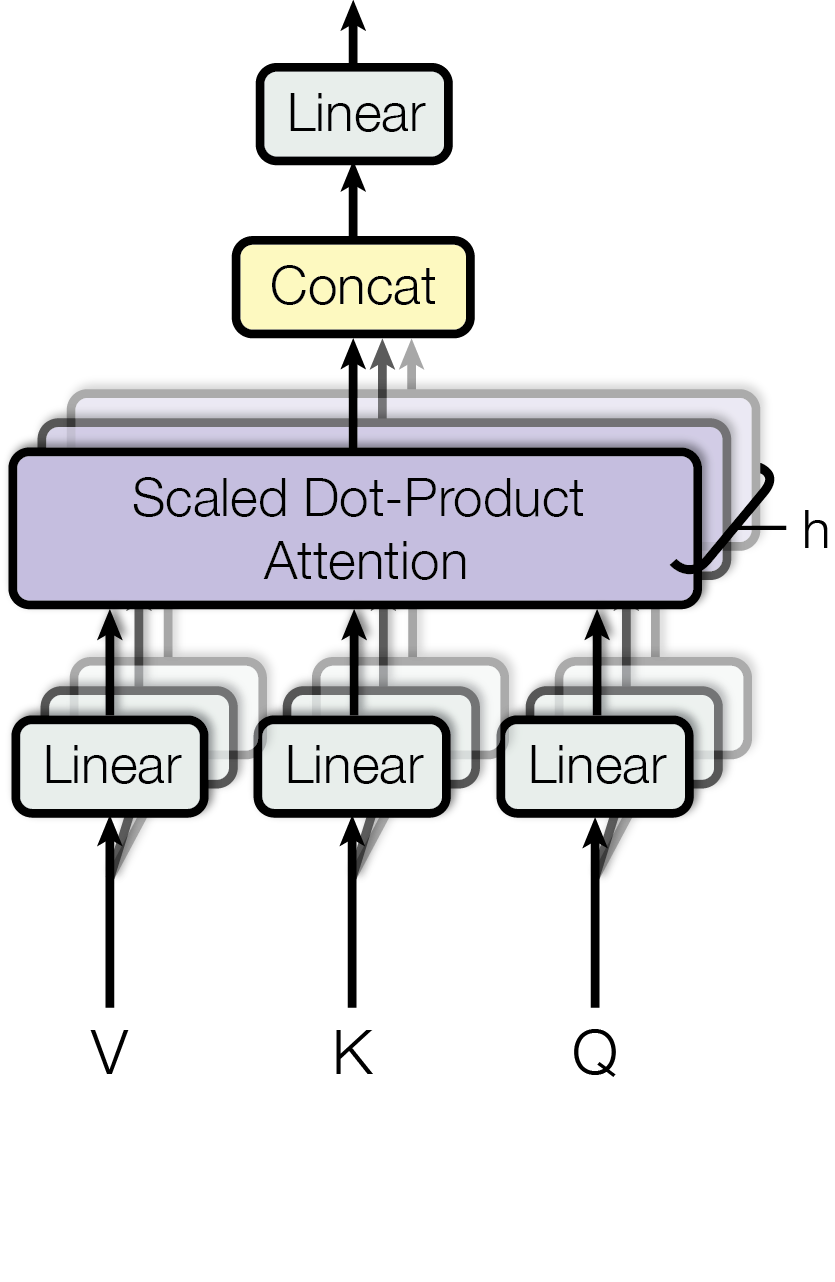
\includegraphics[width=0.3\textwidth]{logos/Multi-head.png}
\caption[Multi-Head Attention mechanism]{Multi-Head Attention consists of several attention layers running in parallel.\cite{vaswani2017attention}}
\label{fig:multi_head_attention}
\end{figure}

In essence, Multi-Head Attention gives the model a broader and more nuanced understanding of the sequence by allowing it to jointly attend to information from different perspectives simultaneously \cite{vaswani2017attention}.

\subsection{The Structure of the Transformer's Encoder}
The Transformer encoder is a stack of identical layers. Each layer is composed of two main sub-layers: a Multi-Head Self-Attention mechanism and a simple, position-wise fully connected Feed-Forward Network (FFN).

Key components of the encoder architecture include:
\begin{itemize}
    \item \textbf{Positional Encoding:} Since the Transformer contains no recurrence or convolution, it has no inherent sense of sequence order. To address this, positional encodings are added to the input embeddings at the bottom of the encoder stack. These are vectors that provide information about the relative or absolute position of tokens in the sequence. The original paper used sine and cosine functions of different frequencies for this purpose \citep{vaswani2017attention}.
    \item \textbf{Feed-Forward Network (FFN):} This sub-layer consists of two linear transformations with a ReLU activation in between: \(\text{FFN}(x) = \max(0, xW_1 + b_1)W_2 + b_2\). It is applied to each position separately and identically, allowing the model to introduce non-linearity and further process the representations from the attention layer \citep{vaswani2017attention}.
    \item \textbf{Residual Connections and Layer Normalization:} Each of the two sub-layers (Multi-Head Attention and FFN) in an encoder layer has a residual connection around it, followed by a layer normalization step. The output of each sub-layer is thus \(\text{LayerNorm}(x + \text{Sublayer}(x))\), where \(\text{Sublayer}(x)\) is the function implemented by the sub-layer itself. These two components are critical for enabling the training of deep Transformer models by stabilizing the learning process and ensuring proper gradient flow \citep{ba2016layer}.
\end{itemize}

\begin{figure}[tb]
\centering
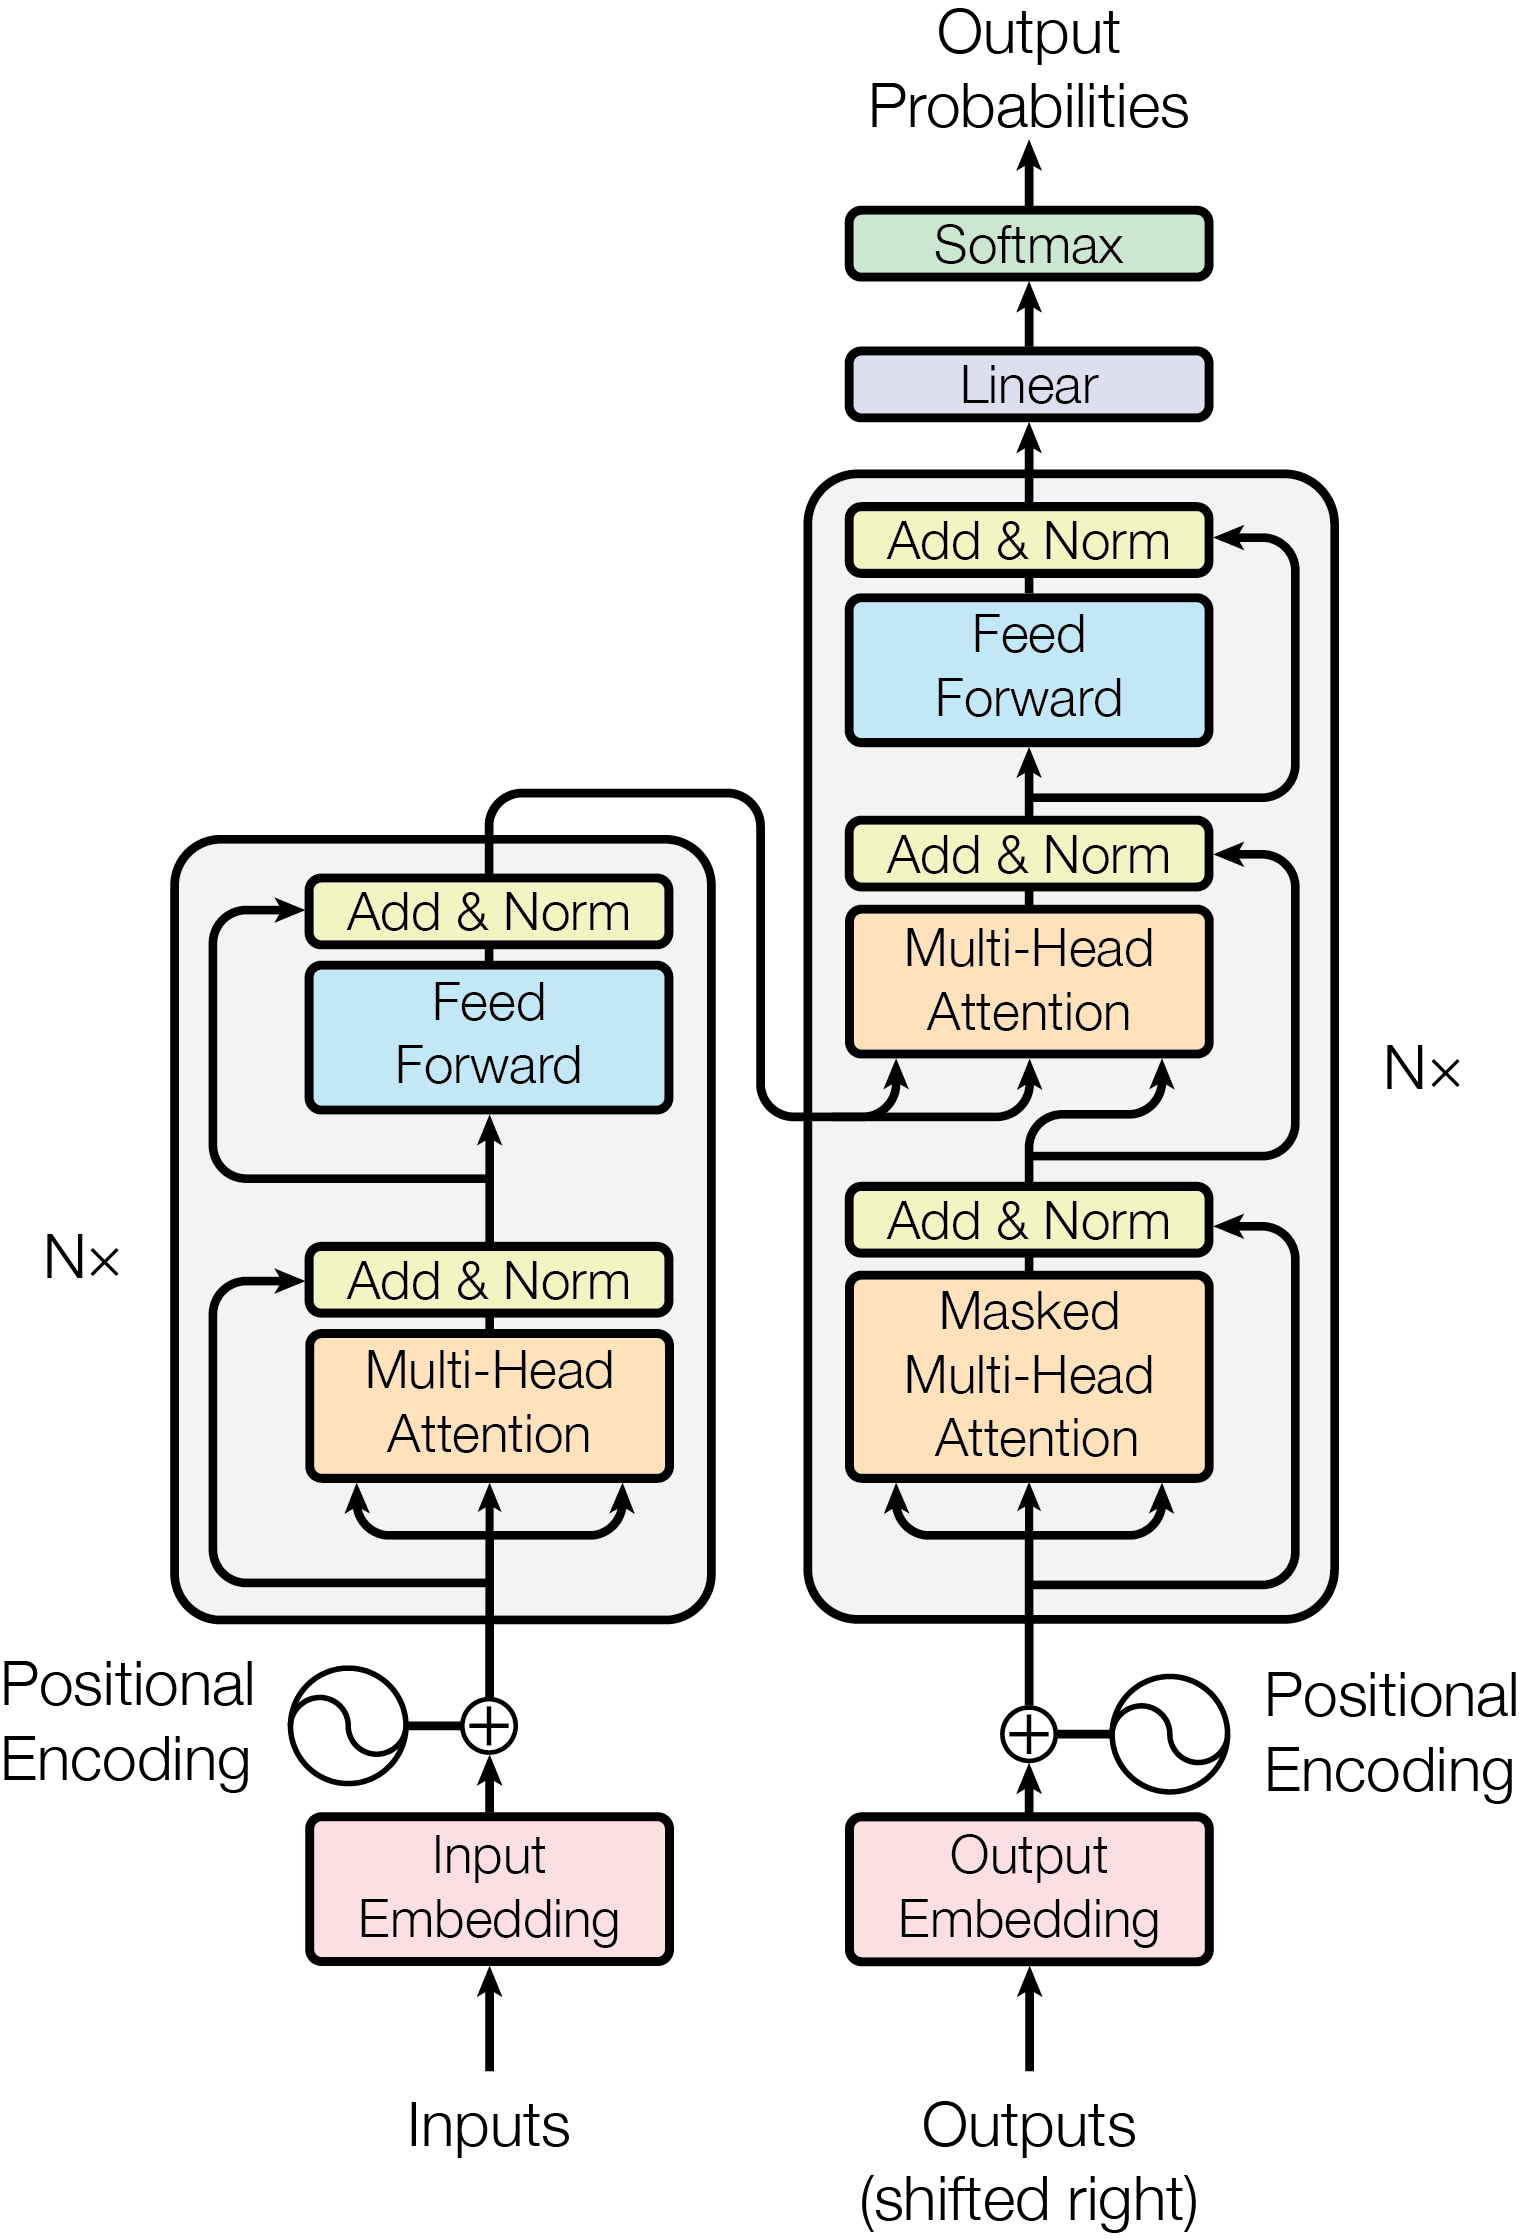
\includegraphics[width=0.5\textwidth]{logos/transformer.png}
\caption[Transformer encoder architecture]{The structure of the Transformer encoder, showing the multi-head self-attention mechanism, feed-forward network, residual connections, and layer normalization components \cite{vaswani2017attention}.}
\label{fig:transformer_encoder}
\end{figure}

As illustrated in Figure~\ref{fig:transformer_encoder}, the Transformer encoder processes input sequences through a stack of identical layers, each containing two main components: a multi-head self-attention mechanism that enables the model to attend to different positions within the sequence, and a position-wise feed-forward network that applies non-linear transformations. The residual connections around each sub-layer, combined with layer normalization, facilitate stable training and effective gradient flow through the deep architecture. This design allows for highly parallelizable computation while capturing complex dependencies across the entire input sequence.



Table~\ref{tab:efficient_attention} summarizes several prominent approaches to reducing the computational complexity of self-attention mechanisms. While standard Transformer attention requires $\mathcal{O}(T^2 d)$ operations for sequence length $T$ and model dimension $d$, these variants achieve sub-quadratic complexity through different approximation strategies. Linformer reduces complexity by projecting the sequence dimension to a lower rank $r$, Performer employs kernel feature maps to linearize attention computation, and Informer uses sparse attention patterns optimized for long-sequence forecasting tasks. These efficiency improvements are particularly relevant for processing long time-series sequences in industrial applications.

\subsection{Positional Encodings and Masking Variants}
While fixed sinusoidal encodings are widely used, alternative schemes exist: \emph{learned} absolute positional embeddings, and \emph{relative} position representations that parameterize pairwise bias as a function of offset, often improving generalization to longer sequences and enabling translation invariance in attention \citep{shaw2018self}. For time-series, seasonal patterns can be injected via multi-scale encodings (e.g., combining periodic sinusoids at different frequencies), and \emph{time-delta} channels can inform the model about irregular sampling.\par
Masking controls information flow. \textbf{Padding masks} prevent attending to padded tokens; \textbf{causal masks} enforce uni-directionality for forecasting/streaming; \textbf{block/local masks} constrain receptive fields to reduce computation while retaining inductive bias for locality.

\subsection{Complexity and Efficient Transformer Variants}
Full self-attention scales as \(\mathcal{O}(T^2 d)\) in time and \(\mathcal{O}(T^2)\) in memory for sequence length \(T\) and model width \(d\), which can be prohibitive for long signals. A line of work proposes sub-quadratic approximations: \textbf{Linformer} projects Keys/Values to a lower rank along the sequence dimension achieving linear complexity in \(T\) \citep{wang2020linformer}; \textbf{Performer} uses randomized feature maps to approximate softmax attention with linear-time kernel attention \citep{choromanski2021rethinking}; \textbf{Informer} exploits ProbSparse attention and top-$k$ queries to reduce cost in long-horizon forecasting \citep{zhou2021informer}. These designs trade a small approximation error for significant speed/memory savings.

\begin{table}[h]
\centering
\caption{Selected efficient attention variants (conceptual summary).}
\label{tab:efficient_attention}
\begin{tabular}{l l l}
\hline
Method & Core idea & Complexity vs. full \\ \hline
Linformer & Low-rank proj. on sequence axis & \(\mathcal{O}(T d r)\) \\
Performer & Kernel feature maps for attention & \(\mathcal{O}(T d^2)\) \\
Informer & ProbSparse/top-$k$ queries & \(\mathcal{O}(T \log T)\) (approx.) \\ \hline
\end{tabular}
\end{table}

\subsection{Architectural Variants for Different Tasks}
\textbf{Encoder-only} stacks (e.g., BERT-style) suit representation learning and classification; \textbf{decoder-only} stacks with causal masks suit autoregressive modeling and forecasting; \textbf{encoder--decoder} designs enable sequence-to-sequence mapping and cross-attention fusion from context to targets. In industrial fault diagnosis, encoder-only Transformers with a classification head are common; for forecasting, causal decoder-only or encoder--decoder architectures are preferred, with appropriate masking.


% --- BEGINNING OF LATEX SECTION ---

% 建议在您的LaTeX文档序言部分确保包含以下包:
% \usepackage{amsmath} % 用于数学环境
% \usepackage{natbib}  % 用于 \citep 等引文命令

\section{Key Technologies in Deep Learning}
\label{sec:key_technologies}

The success of a deep learning model is not solely dependent on its architecture but is profoundly influenced by the synergistic application of several key technologies during the training process. These technologies guide the model's learning, enhance its efficiency, and ensure its ability to generalize to new, unseen data. This section elaborates on the critical components adopted in this research: the loss function chosen to handle data imbalances, the optimization algorithm that drives model convergence, and the regularization techniques employed to combat overfitting.

\subsection{Loss Function: From Cross-Entropy to Focal Loss}
\label{sec:loss_functions}

The loss function serves as the objective for optimization, quantifying the discrepancy between the model's predictions and the ground truth. A well-chosen loss function is paramount for directing the model's learning toward the desired outcome.

\textbf{Cross-Entropy (CE) Loss} is the de facto standard for multi-class classification tasks. It originates from information theory and measures the dissimilarity between two probability distributions: the predicted probability distribution from the model and the true distribution (represented as a one-hot vector). For a single sample, the CE loss is formulated as:
\begin{equation}
\text{CE}(p, y) = - \sum_{i=1}^{C} y_i \log(p_i)
\label{eq:ce_loss}
\end{equation}
where $C$ is the number of classes, $y_i$ is 1 if the sample belongs to class $i$ and 0 otherwise, and $p_i$ is the model's predicted probability for class $i$. While effective in balanced scenarios, CE loss exhibits a significant drawback when faced with \textbf{class imbalance}. In many real-world datasets, such as those in machinery fault diagnosis, normal-condition samples vastly outnumber faulty-condition samples. In such cases, the total loss becomes dominated by the easily classified, high-frequency majority class, leading to a model that is biased and performs poorly on the very classes of interest.

To counteract this, this study employs \textbf{Focal Loss (FL)}, an elegant modification of the standard Cross-Entropy loss \citep{lin2017focal}. Focal Loss dynamically reshapes the loss function to concentrate the training effort on ``hard'' or misclassified examples. It achieves this by introducing a modulating factor to the CE loss:
\begin{equation}
\text{FL}(p_t) = - \alpha_t (1 - p_t)^\gamma \log(p_t)
\label{eq:focal_loss}
\end{equation}
Here, $p_t$ represents the model's estimated probability for the ground-truth class. The key components are:
\begin{enumerate}
    \item \textbf{The Modulating Factor $(1 - p_t)^\gamma$}: This is the core innovation. When a sample is easily classified ($p_t \to 1$), the term $(1 - p_t)$ approaches 0. Raising this to a power $\gamma > 0$ (e.g., $\gamma = 2$) causes the loss contribution of this easy sample to be drastically reduced. Conversely, for a hard sample ($p_t \to 0$), the modulating factor approaches 1, and its loss is preserved. The \textbf{focusing parameter $\gamma$} smoothly adjusts the rate at which easy examples are down-weighted.
    \item \textbf{The Balancing Factor $\alpha_t$}: This is a weighting factor that directly addresses class frequency by assigning a higher weight to minority classes. It provides a static baseline for balancing, which is then dynamically refined by the modulating factor.
\end{enumerate}
By adopting Focal Loss, we equip our model to effectively learn from imbalanced data, ensuring that the rare but crucial fault signatures are not ignored during training.

\subsection{Optimization Algorithm: Adam}
\label{sec:optimizer_adam}

The optimization algorithm is the engine that updates the model's parameters to minimize the loss function. This research utilizes the \textbf{Adam (Adaptive Moment Estimation)} optimizer, a highly effective and widely used algorithm \citep{kingma2014adam}. Adam combines the strengths of two other popular methods: Momentum and RMSprop. It maintains an exponentially decaying average of past gradients (first moment) and past squared gradients (second moment). This allows it to compute individual, adaptive learning rates for different parameters, leading to faster convergence and robust performance across a wide range of deep learning models.

\paragraph{Learning-rate schedules and decoupled weight decay.} Beyond vanilla Adam, \textbf{AdamW} decouples weight decay from the gradient-based update, often yielding better regularization than L2 penalties baked into the loss \citep{loshchilov2019decoupled}. Practical schedules include \textbf{cosine annealing with warm restarts} to escape sharp minima \citep{loshchilov2016sgdr} and the \textbf{OneCycle} policy to traverse a wider range of learning rates/momenta for faster convergence \citep{smith2018superconvergence}. Warmup (a brief linear increase of learning rate at the start) is especially helpful for attention models.

\subsection{Regularization Techniques: Dropout and Weight Decay}
\label{sec:regularization}

A primary challenge in training deep networks is \textbf{overfitting}. To mitigate this risk, we employ two powerful regularization techniques.

\textbf{Dropout} is a method that prevents complex co-adaptations on training data \citep{srivastava2014dropout}. During each training iteration, it randomly sets the outputs of a fraction of neurons to zero. This forces the network to learn more robust features and acts as a form of model averaging.

\paragraph{Data augmentation for time series.} Augmentations such as jittering (Gaussian noise), scaling, magnitude warping, time warping, permutation, and window slicing can improve robustness and reduce overfitting; MixUp/CutMix analogues on temporal signals must be applied with care to preserve label semantics. A recent survey systematizes augmentation choices for time-series deep learning \citep{wen2021time}.

\paragraph{Handling class imbalance beyond Focal Loss.} In addition to Focal Loss, re-sampling (minority oversampling/majority undersampling), synthetic sample generation (e.g., SMOTE \citep{chawla2002smote}), or class-balanced re-weighting by effective number of samples are commonly used. Threshold moving and calibrating decision thresholds on a validation set can further improve minority-class recall without inflating false positives excessively.

\paragraph{Evaluation metrics and reporting.} For multi-class fault diagnosis under imbalance, accuracy alone can be misleading. We report macro-averaged Precision/Recall/F1 and ROC/PR curves. For a class \(c\),
\begin{align}
\mathrm{Precision}_c &= \frac{\mathrm{TP}_c}{\mathrm{TP}_c + \mathrm{FP}_c},\quad
\mathrm{Recall}_c = \frac{\mathrm{TP}_c}{\mathrm{TP}_c + \mathrm{FN}_c},\\
\mathrm{F1}_c &= \frac{2\,\mathrm{Precision}_c\,\mathrm{Recall}_c}{\mathrm{Precision}_c+\mathrm{Recall}_c}.
\end{align}
Macro-averaging treats all classes equally by averaging the per-class scores; micro-averaging aggregates TP/FP/FN across classes before computing the metrics, favoring frequent classes. Confusion matrices complement these metrics by revealing dominant error modes.

\textbf{Weight Decay}, most commonly implemented as \textbf{L2 Regularization}, adds a penalty term to the loss function proportional to the squared magnitude of the model's weights:
\begin{equation}
L_{\text{new}} = L_{\text{original}} + \frac{\lambda}{2} \sum_{w} w^2
\label{eq:l2_reg}
\end{equation}
This penalty encourages the model to find solutions with smaller weights, which typically leads to a less complex model with better generalization performance \citep{goodfellow2016deep}.


\section{Chapter Summary}
\label{sec:related_technologies:summary}

This chapter introduced core sequence models with a focus on LSTMs. We explained why plain RNNs suffer from vanishing/exploding gradients and how the LSTM’s additive cell state with multiplicative gates alleviates this, enabling learning of longer dependencies. The remaining Figure~\ref{fig:lstm_cell_diagram} illustrated the LSTM cell and its forget/input/output gates, serving as a visual complement to the gating equations. We also discussed LSTM strengths and limitations for time-series tasks and the role of Bi-LSTMs when non-causal, bidirectional context is available.
  % Chapter 2: Related Technologies and Theoretical Foundations
\chapter{A Hybrid Transformer-LSTM Model for Fault Diagnosis}
\label{cha:hybrid_model}

\section{Overall Model Architecture}
\label{sec:hybrid_model:architecture}

\subsection{Model Overview and Data Flow}
The core of this research is the Transformer-LSTM Model, a deep learning hybrid architecture specifically designed to extract multi-level temporal features from sequential data for classification tasks. This approach simultaneously leverages the global attention capabilities of Transformer networks with the sequential modeling strengths of LSTM architectures, creating a powerful framework for fault diagnosis applications. Figure~\ref{fig:hybrid_architecture} illustrates the complete architecture of our proposed model, which processes data through two parallel feature extraction pathways before fusing them for final classification.


The data processing pipeline operates as follows:
\begin{figure}[p]
\centering
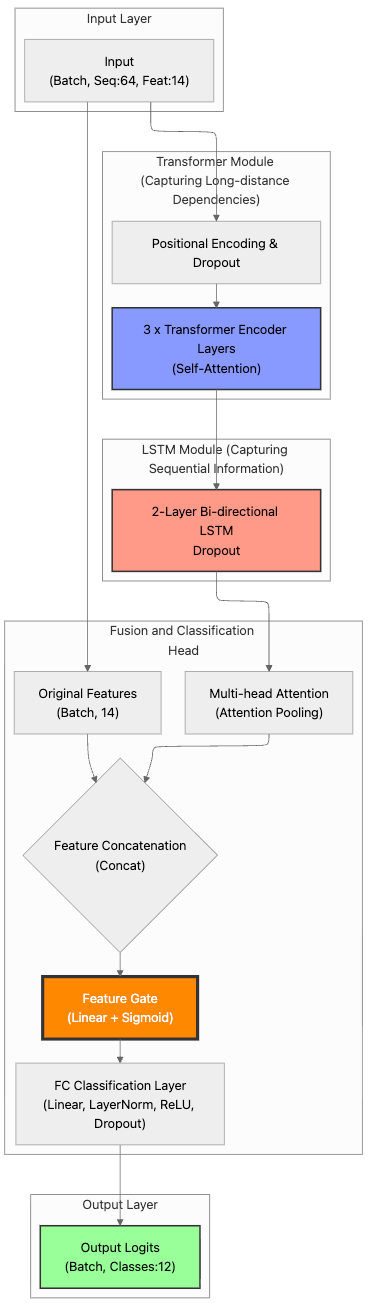
\includegraphics[width=0.5\textwidth]{logos/transformer-lstm.png}
\caption{Transformer-LSTM Model Architecture Overview: The diagram shows the complete data flow from input time-series data through various processing stages including input projection, positional encoding, Transformer encoder, bidirectional LSTM, multi-head attention, and feature fusion, ultimately leading to fault classification.}
\label{fig:hybrid_architecture}
\end{figure}

\begin{enumerate}
    \item \textbf{Input Layer}: The model receives raw time-series data, with a shape of \texttt{[Batch, Seq:64, Feat:14]}, representing a batch of sequences, each with a length of 64 time steps and 14 features per step.
    \item \textbf{Input Processing - Dual Pathway Architecture}: The raw input data is duplicated and processed through two parallel pathways:
    \begin{itemize}
    \item \textbf{Main Processing Path}: The raw input passes through a linear projection layer and layer normalization, mapping the feature dimension to a space suitable for Transformer processing while ensuring training stability.
    
    \item \textbf{Skip Connection Path}: The final time-step features of the raw input are preserved as a skip connection, directly passed to the subsequent feature fusion stage to retain critical information from the original signal.
    \end{itemize}
    
    \item \textbf{Positional Encoding}: Positional information is added to the normalized input of the main processing path to provide sequence order awareness for the Transformer component.

    \item \textbf{Transformer Encoder (Global Feature Extraction)}: The encoded input is processed by \textbf{3 stacked Transformer Encoder Layers}, which use multi-head self-attention to capture long-range dependencies and global context across the entire sequence. This stage provides a rich global representation that forms the foundation for subsequent processing.

    \item \textbf{Bidirectional LSTM (Temporal Refinement)}: The Transformer output is then fed into a \textbf{2-Layer Bi-directional LSTM} network with dropout regularization. This stage refines the global features by incorporating local temporal patterns and sequential dependencies, processing information from both past and future contexts at each time step.

    \item \textbf{Self-Attention Pooling}: The LSTM output sequence is processed by a \textbf{Multi-head Attention} mechanism that acts as an attention pooling layer. This learns to weigh the importance of different time steps and aggregates the sequence into a single, fixed-size context vector that captures the most critical temporal information.

    \item \textbf{Feature Fusion and Gate Mechanism}: The model combines features from two key sources:
    \begin{enumerate}
    \item The attention-pooled LSTM output vector that captures processed temporal patterns
    \item The final time-step features from the original projected input (skip connection) that preserve raw signal characteristics
    \end{enumerate}
    These features are concatenated and passed through a \textbf{Feature Gate} composed of a linear layer followed by sigmoid activation, which adaptively controls information flow by selectively emphasizing the most relevant features.

    \item \textbf{Classification Head}: The gated feature vector is processed through a fully connected classification layer with layer normalization, ReLU activation, and dropout for regularization. This maps the fused high-level representation to the final 12-class output space.

    \item \textbf{Output Layer}: The model produces \textbf{Output Logits} with shape \texttt{[Batch, Classes:12]}, providing raw scores for each fault category. These logits can be passed through a softmax function to obtain class probabilities for final predictions.
\end{enumerate}




\subsection{Core Design Philosophy: Divide and Conquer, Leveraging Strengths}

The core design philosophy of this model architecture is "divide and conquer, leveraging individual strengths," which involves fully utilizing the respective advantages of the Transformer and LSTM and combining them through an effective fusion mechanism to achieve a more comprehensive and robust analysis of time-series data.

\begin{itemize}
    \item \textbf{Transformer: Global Dependencies and Parallel Processing}
    \begin{itemize}
        \item \textbf{Strengths:} The Transformer, through its self-attention mechanism, can efficiently capture long-range dependencies between any two positions in a sequence, regardless of their distance \citep{vaswani2017attention, shaw2018self}. This is crucial for understanding global patterns and context. Furthermore, its parallel computation capability provides a significant efficiency advantage when processing long sequences, addressing limitations of sequential models like traditional RNNs \citep{pascanu2013difficulty}.
        \item \textbf{Role:} In this architecture, the Transformer is primarily responsible for performing global feature extraction and contextual modeling on the input sequence at an early stage, providing a representation enriched with global information for the subsequent LSTM layer.
    \end{itemize}
    \item \textbf{LSTM: Local Temporal Patterns and Memory}
    \begin{itemize}
        \item \textbf{Strengths:} As a recurrent neural network, the LSTM possesses excellent memory capabilities for processing sequential data, enabling it to effectively learn and remember local temporal patterns and short-term dependencies \citep{hochreiter1997long}. The bidirectional nature further enhances this ability by allowing it to consider both past and future information, making it particularly suitable for time-series analysis in fault diagnosis applications \citep{filonov2016multivariateindustrialtimeseries, zhao2019deep}.
        \item \textbf{Role:} The role of the LSTM in this architecture is to further refine and capture more fine-grained local temporal features and dynamic changes, building upon the global features extracted by the Transformer. It deeply models the sequential nature of the information.
    \end{itemize}
    \item \textbf{Fusion Mechanism: Synergy and Information Integration}
    \begin{itemize}
        \item \textbf{Strengths:} A simple serial connection might not fully realize the synergy between the two models. This model implements a more intelligent information integration by introducing another attention mechanism after the LSTM output and incorporating a gated fusion with the original input features. This fusion not only combines the global perspective of the Transformer and the local insights of the LSTM but also adaptively adjusts the importance of features from different sources via the gating mechanism, ensuring effective information transfer and complementarity.
        \item \textbf{Role:} The fusion mechanism ensures that the model can learn from different levels and types of features, thereby constructing a more powerful and discriminative feature representation that ultimately enhances the overall performance of the model.
    \end{itemize}
\end{itemize}

Through this "divide and conquer, leveraging strengths" design, the Transformer-LSTM Model can effectively process complex time-series data, capturing both long-range dependencies and global context while finely modeling local temporal patterns, ultimately achieving high-precision classification.

\subsection{Mathematical Formulation}
\label{subsec:mathematical_formulation}

To provide a formal mathematical description of the model architecture, we define the sequential transformations applied to the input data. Given an input time-series sequence $X \in \mathbb{R}^{B \times L \times D}$, where $B$ represents the batch size, $L$ denotes the sequence length (typically 64), and $D$ is the feature dimension (14 for our fault diagnosis dataset), the model processes the data through the following stages:

\begin{align}
X_{\text{proj}} = \text{LayerNorm}(\text{Linear}(X)) \label{eq:input_projection} \\
X_{\text{pos}} = X_{\text{proj}} + \text{PE}(L) \label{eq:positional_encoding} \\
H_{\text{trans}} = \text{TransformerEncoder}(X_{\text{pos}}) \label{eq:transformer} \\
H_{\text{lstm}} = \text{BiLSTM}(H_{\text{trans}}) \label{eq:lstm} \\
H_{\text{attn}} = \text{MultiHeadAttention}(H_{\text{lstm}}, H_{\text{lstm}}, H_{\text{lstm}}) \label{eq:attention} \\
H_{\text{fused}} = \text{FeatureGate}([H_{\text{attn}}[-1], X_{\text{proj}}[-1]]) \label{eq:fusion} \\
\hat{y} = \text{FC}(H_{\text{fused}}) \label{eq:output}
\end{align}

where $\text{PE}(L)$ represents the sinusoidal positional encoding, $H_{\text{attn}}[-1]$ and $X_{\text{proj}}[-1]$ denote the final time-step features from the attention output and projected input respectively, and $\text{FC}$ represents the fully connected classification layers.

The feature gating mechanism is defined as:
\begin{align}
\text{FeatureGate}(h_{\text{attn}}, h_{\text{orig}}) = h_{\text{attn}} \odot \sigma(\text{Linear}([h_{\text{attn}}, h_{\text{orig}}])) \label{eq:gate}
\end{align}

where $\odot$ denotes element-wise multiplication, $\sigma$ is the sigmoid activation function, and $[\cdot, \cdot]$ represents concatenation.

\subsection{Model Configuration and Parameters}
\label{subsec:model_configuration}

Table~\ref{tab:model_config} presents the specific configuration parameters used in our Transformer-LSTM Model implementation, optimized for fault diagnosis tasks.

\begin{table}[htbp]
\centering
\caption{TransformerLSTMModel Configuration Parameters}
\label{tab:model_config}
\begin{tabular}{|l|c|l|}
\hline
\textbf{Component} & \textbf{Parameter} & \textbf{Value} \\
\hline
\multirow{2}{*}{Input Processing} & Input Dimension & 14 \\
 & Sequence Length & 64 \\
\hline
\multirow{4}{*}{Transformer Encoder} & Hidden Dimension & 336 \\
 & Number of Layers & 3 \\
 & Number of Attention Heads & 2 \\
 & Dropout Rate & 0.22 \\
\hline
\multirow{3}{*}{LSTM Component} & Hidden Units & 336 \\
 & Number of Layers & 2 \\
 & Bidirectional & True \\
\hline
\multirow{2}{*}{Attention Mechanism} & Embed Dimension & 672 (336$\times$2) \\
 & Number of Heads & 2 \\
\hline
\multirow{3}{*}{Classification Layers} & FC1 Dimension & 336 \\
 & FC2 Dimension & 168 \\
 & Output Classes & 12 \\
\hline
\multirow{2}{*}{Training} & Learning Rate & 0.0006 \\
 & Weight Decay & 6$\times$10$^{-5}$ \\
\hline
\end{tabular}
\end{table}

The model contains approximately 2.1 million trainable parameters, making it computationally efficient while maintaining high representational capacity for complex fault pattern recognition.

\subsection{Computational Complexity Analysis}
\label{subsec:complexity_analysis}

The computational complexity of the Transformer-LSTM Model can be analyzed by examining each component:

\begin{itemize}
    \item \textbf{Transformer Encoder}: The self-attention mechanism has complexity $O(L^2 \cdot D)$ for sequence length $L$ and hidden dimension $D$. With 3 layers, the total complexity is $O(3 \cdot L^2 \cdot D)$.
    
    \item \textbf{LSTM Processing}: The bidirectional LSTM with 2 layers has complexity $O(2 \cdot L \cdot D^2)$ for sequential processing.
    
    \item \textbf{Multi-head Attention}: The final attention layer adds $O(L^2 \cdot D_{\text{lstm}})$ complexity, where $D_{\text{lstm}} = 2D$ for bidirectional LSTM.
    
    \item \textbf{Overall Complexity}: The total computational complexity is $O(L^2 \cdot D + L \cdot D^2)$, which scales quadratically with sequence length but remains manageable for our typical sequence length of 64.
\end{itemize}

For our specific configuration with $L = 64$ and $D = 336$, this results in efficient processing suitable for real-time fault diagnosis applications.

\section{Data Preprocessing Module}
\label{sec:hybrid_model:preprocessing}

The data preprocessing module is a critical component that prepares raw machine fault data for effective learning by the hybrid model. This module encompasses several key operations designed to enhance data quality, increase dataset diversity, and ensure optimal model performance \citep{liu2018artificial}.

\subsection{Data Loading and Class Merging}
\label{subsec:data_loading}

Our fault diagnosis system processes 12 distinct fault categories as defined in the label set:
\begin{align}
\mathcal{L} = \{\text{good}, \text{JERK\_A}, \text{BACKLASH\_X}, \text{JERK\_ALL}, \nonumber \\
\text{ALL\_processed}, \text{JERK\_X}, \text{BACKLASH\_Y}, \text{BS\_XY}, \nonumber \\
\text{BS\_X}, \text{JERK\_Y}, \text{JERK\_B}, \text{BS\_Y}\}
\end{align}

The preprocessing module consolidates multiple ``good'' condition files (good\_1, good\_2, good\_3) into a single normal operating class, ensuring balanced representation of healthy machine states across different operational scenarios.

\subsection{Sliding Window Sequence Generation}
\label{subsec:sliding_window}

To capture temporal patterns essential for fault diagnosis, the preprocessing module implements an adaptive sliding window approach:

\begin{itemize}
    \item \textbf{Window Size}: Fixed at 64 time steps, optimized for capturing both short-term transients and medium-term fault development patterns
    \item \textbf{Sampling Strategy}: For longer sequences (> 192 samples), up to 800 windows are randomly sampled per file to maximize data utilization while maintaining computational efficiency
    \item \textbf{Overlap Management}: Random starting positions prevent systematic bias and ensure diverse temporal perspectives of fault patterns
\end{itemize}

The sliding window extraction process can be formalized as:
\begin{align}
W_i = X[s_i : s_i + L] \quad \text{for } i = 1, 2, \ldots, N_w \\
s_i \sim \text{Uniform}(0, T - L)
\end{align}

where $W_i$ represents the $i$-th window, $s_i$ is the starting position, $L = 64$ is the window length, $T$ is the total sequence length, and $N_w$ is the number of windows extracted.

\subsection{Data Normalization and Scaling}
\label{subsec:normalization}

To ensure numerical stability and convergence, the preprocessing module employs robust scaling techniques:

\begin{itemize}
    \item \textbf{Robust Scaler}: Applied to handle outliers and maintain signal characteristics across different sensors and operational conditions
    \item \textbf{Channel-wise Normalization}: Each of the 14 sensor channels is independently scaled to preserve relative signal relationships
    \item \textbf{Preservation of Temporal Dependencies}: Scaling parameters are computed globally but applied consistently to maintain temporal coherence
\end{itemize}

The robust scaling transformation is defined as:
\begin{equation}
X_{\text{scaled}} = \frac{X - \text{median}(X)}{\text{IQR}(X)}
\end{equation}

where IQR represents the interquartile range, providing robustness against outliers commonly present in industrial sensor data.

\subsection{Data Augmentation Strategies}
\label{subsec:data_augmentation}

To enhance model generalization and address class imbalance, the preprocessing module incorporates several augmentation techniques:

\begin{enumerate}
    \item \textbf{Amplitude Scaling}: Random scaling factors $\alpha \sim \mathcal{U}(0.85, 1.15)$ applied channel-wise with 70\% probability
    \item \textbf{Gaussian Noise Injection}: Low-level noise $\epsilon \sim \mathcal{N}(0, 0.01\sigma^2)$ added to simulate sensor uncertainty  
    \item \textbf{Time Shifting}: Minimal temporal shifts to account for synchronization variations
    \item \textbf{Channel Dropout}: Random masking of sensor channels to improve robustness against sensor failures
\end{enumerate}

These augmentation strategies are applied probabilistically during training to increase dataset diversity while preserving the fundamental characteristics of fault signatures.

\section{Transformer Feature Extraction Component}
\label{sec:hybrid_model:transformer_component}

The Transformer component serves as the global feature extraction backbone of our hybrid architecture, leveraging self-attention mechanisms to capture long-range dependencies and global patterns within the fault signature sequences \citep{vaswani2017attention, zhou2021informer}.

\subsection{Input Processing and Positional Encoding}
\label{subsec:input_processing}

The Transformer component begins with input processing that prepares the sequential data for attention-based feature extraction:

\begin{enumerate}
    \item \textbf{Input Projection}: A linear transformation projects the 14-dimensional sensor readings into the model's hidden dimension:
    \begin{equation}
X_{\text{proj}} = X \cdot W_{\text{proj}} + b_{\text{proj}}
\end{equation}

    where $W_{\text{proj}} \in \mathbb{R}^{14 \times 336}$ and $X_{\text{proj}} \in \mathbb{R}^{B \times 64 \times 336}$.
    
    \item \textbf{Layer Normalization}: Applied to stabilize training and improve convergence:
    \begin{equation}
X_{\text{norm}} = \text{LayerNorm}(X_{\text{proj}})
\end{equation}
    
    \item \textbf{Sinusoidal Positional Encoding}: Since Transformers lack inherent sequential processing, positional information is added:
    \begin{align}
PE_{(pos, 2i)} = \sin\left(\frac{pos}{10000^{2i/d_{\text{model}}}}\right) \\
PE_{(pos, 2i+1)} = \cos\left(\frac{pos}{10000^{2i/d_{\text{model}}}}\right)
\end{align}

    where $pos$ is the position, $i$ is the dimension index, and $d_{\text{model}} = 336$.
\end{enumerate}

\subsection{Multi-Head Self-Attention Mechanism}
\label{subsec:self_attention}

The core of the Transformer component employs multi-head self-attention to capture complex relationships between different time steps in the fault signature:

\begin{align}
\text{Attention}(Q, K, V) = \text{softmax}\left(\frac{QK^T}{\sqrt{d_k}}\right)V \\
\text{MultiHead}(X) = \text{Concat}(\text{head}_1, \ldots, \text{head}_h)W^O
\end{align}

where each attention head is computed as:
\begin{equation}
\text{head}_i = \text{Attention}(XW_i^Q, XW_i^K, XW_i^V)
\end{equation}

With 2 attention heads and $d_k = d_v = 168$, the mechanism enables the model to attend to different types of temporal relationships simultaneously.

\subsection{Feed-Forward Networks and Residual Connections}
\label{subsec:ffn_residual}

Each Transformer layer incorporates position-wise feed-forward networks with residual connections:

\begin{equation}
\text{FFN}(x) = \text{ReLU}(xW_1 + b_1)W_2 + b_2
\end{equation}

\begin{equation}
\text{TransformerLayer}(x) = \text{LayerNorm}(x + \text{FFN}(\text{LayerNorm}(x + \text{MultiHead}(x))))
\end{equation}

The residual connections facilitate gradient flow during training, while layer normalization ensures stable optimization dynamics.

\subsection{Global Context Extraction}
\label{subsec:global_context}

Through 3 stacked Transformer layers, the component progressively builds representations that capture:

\begin{itemize}
    \item \textbf{Short-term Correlations}: Direct dependencies between adjacent time steps
    \item \textbf{Medium-term Patterns}: Periodic behaviors and cyclic fault signatures  
    \item \textbf{Long-range Dependencies}: Global trends and slowly evolving fault characteristics
    \item \textbf{Cross-channel Interactions}: Relationships between different sensor modalities
\end{itemize}

The parallel processing capability of the Transformer enables efficient computation while maintaining the ability to model complex temporal interactions essential for accurate fault diagnosis.

\section{LSTM Sequence Modeling Component}
\label{sec:hybrid_model:lstm_component}

The LSTM component operates on the globally-enhanced representations from the Transformer, focusing on sequential pattern extraction and local temporal dependency modeling. This component is specifically designed to capture the recurrent nature of fault evolution and machine degradation processes \citep{hochreiter1997long, filonov2016multivariateindustrialtimeseries}.

\subsection{Bidirectional LSTM Architecture}
\label{subsec:bilstm_architecture}

The LSTM component employs a bidirectional architecture with 2 layers, each containing 336 hidden units. The bidirectional design enables the model to process information from both past and future contexts:

\begin{align}
\overrightarrow{h}_t = \text{LSTM}_{\text{forward}}(x_t, \overrightarrow{h}_{t-1}) \\
\overleftarrow{h}_t = \text{LSTM}_{\text{backward}}(x_t, \overleftarrow{h}_{t+1}) \\
h_t = [\overrightarrow{h}_t; \overleftarrow{h}_t]
\end{align}

where $h_t \in \mathbb{R}^{672}$ represents the concatenated bidirectional hidden state at time step $t$.

\subsection{Temporal Pattern Extraction}
\label{subsec:temporal_patterns}

The LSTM component excels at capturing several types of temporal patterns crucial for fault diagnosis:

\begin{itemize}
    \item \textbf{Sequential Dependencies}: The recurrent connections enable modeling of how current machine states depend on previous conditions
    \item \textbf{Fault Evolution Patterns}: The cell state mechanism allows the model to track gradual fault development over time
    \item \textbf{Local Temporal Features}: Short-term variations and transient behaviors that may indicate incipient faults
    \item \textbf{Memory of Critical Events}: The forget and input gates enable selective retention of important fault-related information
\end{itemize}

\subsection{Layer Stacking and Regularization}
\label{subsec:lstm_regularization}

The 2-layer LSTM configuration provides hierarchical feature extraction:

\begin{itemize}
    \item \textbf{First Layer}: Captures basic sequential patterns and low-level temporal dependencies
    \item \textbf{Second Layer}: Extracts higher-level temporal abstractions and complex sequential relationships
    \item \textbf{Dropout Regularization}: Applied between layers (rate = 0.22) to prevent overfitting while preserving temporal coherence
    \item \textbf{Gradient Clipping}: Implemented to address potential vanishing/exploding gradient issues commonly encountered in recurrent networks \citep{pascanu2013difficulty}
\end{itemize}

The output of the LSTM component, $H_{\text{lstm}} \in \mathbb{R}^{B \times 64 \times 672}$, provides temporally-aware representations that complement the global features extracted by the Transformer component.

\section{Adaptive Feature Fusion Strategy}
\label{sec:hybrid_model:fusion_strategy}

The feature fusion strategy represents a critical innovation in our hybrid architecture, intelligently combining representations from different processing stages to create a comprehensive feature vector for fault classification. This section details the multi-stage fusion mechanism that enhances the model's discriminative capability.

\subsection{Multi-Head Attention on LSTM Output}
\label{subsec:lstm_attention}

Before fusion, the LSTM output undergoes an additional attention mechanism to further refine the temporal features:

\begin{align}
H_{\text{attn}} = \text{MultiHeadAttention}(H_{\text{lstm}}, H_{\text{lstm}}, H_{\text{lstm}}) \\
= \text{Concat}(\text{head}_1, \ldots, \text{head}_2)W^O
\end{align}

This attention layer operates with 2 heads on the 672-dimensional LSTM output, enabling the model to focus on the most relevant temporal features for classification. The attention mechanism helps identify critical time steps that contain the most discriminative fault information.

\subsection{Feature Extraction for Fusion}
\label{subsec:feature_extraction_fusion}

The fusion process combines features from two distinct processing pathways:

\begin{enumerate}
    \item \textbf{Processed Pathway}: The final time-step output from the attention-enhanced LSTM:
    \begin{equation}
f_{\text{processed}} = H_{\text{attn}}[:, -1, :] \in \mathbb{R}^{B \times 672}
\end{equation}
    
    \item \textbf{Direct Pathway}: The final time-step from the original projected input:
    \begin{equation}
f_{\text{original}} = X_{\text{proj}}[:, -1, :] \in \mathbb{R}^{B \times 336}
\end{equation}
\end{enumerate}

This dual-pathway approach ensures that both highly processed features and direct input information contribute to the final decision.

\subsection{Gated Fusion Mechanism}
\label{subsec:gated_fusion}

The core innovation lies in the adaptive gating mechanism that intelligently weights the contribution of different feature sources:

\begin{align}
f_{\text{concat}} = [f_{\text{processed}}; f_{\text{original}}] \in \mathbb{R}^{B \times 1008} \\
g = \sigma(W_g \cdot f_{\text{concat}} + b_g) \in \mathbb{R}^{B \times 672} \\
f_{\text{fused}} = f_{\text{processed}} \odot g
\end{align}

where $W_g \in \mathbb{R}^{672 \times 1008}$ is the linear transformation matrix that maps the concatenated 1008-dimensional features to 672-dimensional gate values, $\sigma$ is the sigmoid activation function, and $\odot$ represents element-wise multiplication. The bias term $b_g \in \mathbb{R}^{672}$ provides learned offsets for each gate dimension.

\subsection{Adaptive Weight Learning}
\label{subsec:adaptive_weights}

The gating mechanism provides several advantages:

\begin{itemize}
    \item \textbf{Adaptive Importance}: The gate values $g$ are learned during training, allowing the model to automatically determine the relative importance of processed vs. original features
    \item \textbf{Context-Dependent Fusion}: Different fault types may require different balances between global context (Transformer) and local patterns (LSTM)
    \item \textbf{Information Preservation}: The residual-like structure ensures that critical information from the original input is preserved through the fusion process
    \item \textbf{Gradient Flow}: The gating mechanism facilitates better gradient propagation during backpropagation
\end{itemize}

\subsection{Fusion Strategy Benefits}
\label{subsec:fusion_benefits}

The adaptive fusion strategy addresses several challenges in fault diagnosis:

\begin{enumerate}
    \item \textbf{Multi-Scale Feature Integration}: Combines global (Transformer) and local (LSTM) temporal features
    \item \textbf{Information Bottleneck Mitigation}: Preserves important information that might be lost in deep processing
    \item \textbf{Fault-Specific Adaptation}: Different fault types can utilize different feature combinations optimally
    \item \textbf{Robustness Enhancement}: The dual-pathway design provides redundancy against feature degradation
\end{enumerate}

The fused feature vector $f_{\text{fused}} \in \mathbb{R}^{B \times 672}$ serves as input to the final classification layers, containing rich representations that capture both global context and local temporal patterns essential for accurate fault diagnosis. This 672-dimensional representation is subsequently mapped to the final classification output through additional fully-connected layers.

\section{Model Training and Optimization Strategy}
\label{sec:hybrid_model:training_optimization}

The training strategy for the Transformer-LSTM Model incorporates several advanced optimization techniques designed to achieve stable convergence, prevent overfitting, and maximize performance on the fault diagnosis task.

\subsection{Loss Function and Class Balancing}
\label{subsec:loss_function}

Given the inherent class imbalance in fault diagnosis datasets, we employ a Focal Loss function combined with class weighting:

\begin{align}
\text{FL}(p_t) = -\alpha_t(1-p_t)^{\gamma}\log(p_t) \\
\alpha_t = \begin{cases} 
\alpha & \text{if } y = 1 \\
1-\alpha & \text{otherwise}
\end{cases}
\end{align}

where $p_t$ is the model's estimated probability for the ground truth class, $\alpha$ balances the importance of positive/negative examples, and $\gamma = 2.0$ is the focusing parameter that down-weights well-classified examples.

Class weights are computed using inverse frequency weighting:
\begin{equation}
w_i = \frac{n_{\text{total}}}{n_{\text{classes}} \times n_i}
\end{equation}

where $n_i$ is the number of samples in class $i$.

\subsection{Optimizer Configuration}
\label{subsec:optimizer}

The model employs the AdamW optimizer \citep{loshchilov2019decoupled} with the following configuration:

\begin{itemize}
    \item \textbf{Learning Rate}: $\eta = 6 \times 10^{-4}$
    \item \textbf{Weight Decay}: $\lambda = 6 \times 10^{-5}$
    \item \textbf{Betas}: $\beta_1 = 0.9, \beta_2 = 0.999$
    \item \textbf{Epsilon}: $\epsilon = 10^{-8}$
\end{itemize}

AdamW decouples weight decay from gradient-based updates, providing better generalization \citep{loshchilov2019decoupled}:
\begin{align}
m_t = \beta_1 m_{t-1} + (1-\beta_1)g_t \\
v_t = \beta_2 v_{t-1} + (1-\beta_2)g_t^2 \\
\theta_t = \theta_{t-1} - \eta\left(\frac{m_t}{\sqrt{v_t} + \epsilon} + \lambda\theta_{t-1}\right)
\end{align}

\subsection{Learning Rate Scheduling}
\label{subsec:lr_scheduling}

A sophisticated learning rate schedule combines warmup and cosine annealing \citep{loshchilov2016sgdr, smith2018superconvergence}:

\begin{enumerate}
    \item \textbf{Warmup Phase} (epochs 1-10):
    \begin{equation}
\eta_t = \eta_{\text{start}} + \frac{(\eta_{\text{max}} - \eta_{\text{start}}) \times t}{T_{\text{warmup}}}
\end{equation}

    where $\eta_{\text{start}} = 1.8 \times 10^{-5}$ and $\eta_{\text{max}} = 6 \times 10^{-4}$.
    
    \item \textbf{Cosine Annealing} (epochs 11-150):
    \begin{equation}
\eta_t = \eta_{\text{min}} + \frac{1}{2}(\eta_{\text{max}} - \eta_{\text{min}})\left(1 + \cos\left(\frac{t - T_{\text{warmup}}}{T_{\text{max}} - T_{\text{warmup}}}\pi\right)\right)
\end{equation}
\end{enumerate}

\subsection{Regularization Techniques}
\label{subsec:regularization}

Multiple regularization strategies prevent overfitting:

\begin{itemize}
    \item \textbf{Dropout}: Applied with rate 0.22 in Transformer and LSTM layers \citep{srivastava2014dropout}
    \item \textbf{Layer Normalization}: Stabilizes training and acts as implicit regularization \citep{ba2016layer}
    \item \textbf{Weight Decay}: L2 regularization through AdamW optimizer
    \item \textbf{Early Stopping}: Training halts when validation loss stops improving for 30 epochs
    \item \textbf{Gradient Clipping}: Prevents exploding gradients with maximum norm of 1.0
\end{itemize}

\subsection{Advanced Training Techniques}
\label{subsec:advanced_training}

Several advanced techniques enhance training efficiency and model performance:

\begin{enumerate}
    \item \textbf{Mixed Precision Training}: Utilizes automatic mixed precision (AMP) to reduce memory usage and accelerate training on CUDA devices \citep{micikevicius2017mixed}
    
    \item \textbf{Data Augmentation}: Applied during training with probability-based augmentation including techniques commonly used in time-series analysis \citep{wen2021time}:
    \begin{itemize}
        \item Amplitude scaling: $x' = x \times \alpha, \alpha \sim \mathcal{U}(0.85, 1.15)$
        \item Gaussian noise: $x' = x + \epsilon, \epsilon \sim \mathcal{N}(0, 0.01\sigma^2)$
        \item Channel dropout: Random masking of sensor channels
    \end{itemize}
    
    \item \textbf{Batch Size Optimization}: Uses batch size of 64 to balance memory efficiency and gradient stability
    
    \item \textbf{Model Checkpointing}: Saves best model based on validation performance for early stopping recovery
\end{enumerate}

\subsection{Training Configuration Summary}
\label{subsec:training_summary}

Table~\ref{tab:training_config} summarizes the complete training configuration used for the Transformer-LSTM Model.

\begin{table}[h]
\centering
\caption{Training Configuration Parameters}
\label{tab:training_config}
\begin{tabular}{|l|c|}
\hline
\textbf{Parameter} & \textbf{Value} \\
\hline
Total Epochs & 150 \\
Batch Size & 64 \\
Learning Rate (max) & $6 \times 10^{-4}$ \\
Weight Decay & $6 \times 10^{-5}$ \\
Warmup Epochs & 10 \\
Early Stopping Patience & 30 \\
Dropout Rate & 0.22 \\
Gradient Clipping & 1.0 \\
Loss Function & Focal Loss ($\gamma=2.0$) \\
Data Split & 70\%/15\%/15\% (Train/Val/Test) \\
\hline
\end{tabular}
\end{table}

This comprehensive training strategy ensures robust optimization while maintaining generalization capability for effective fault diagnosis performance.

\section{Chapter Summary}
\label{sec:hybrid_model:summary}

This chapter presents a novel Transformer-LSTM hybrid architecture for industrial fault diagnosis, integrating global context awareness with local temporal pattern recognition.

The core innovation lies in the adaptive feature fusion strategy that dynamically balances Transformer-derived global features and LSTM-captured sequential patterns through a learnable gating mechanism.

Key technical contributions include:

\begin{enumerate}
    \item \textbf{Dual-pathway processing}: Preserving both deep-extracted and original features through parallel processing pathways
    \item \textbf{Multi-head attention enhancement}: Applying multi-head attention on LSTM outputs for enhanced temporal feature refinement
    \item \textbf{Comprehensive preprocessing}: Implementing sliding window generation and data augmentation for robust feature extraction
    \item \textbf{Optimized training strategy}: Combining focal loss, AdamW optimization, and cosine annealing scheduling for stable convergence
\end{enumerate}

The model achieves multi-scale temporal analysis with computational efficiency ($O(L^2 \cdot D + L \cdot D^2)$) and approximately 2.1M parameters, making it suitable for real-time industrial applications.

Its scalability allows adaptation to various fault diagnosis scenarios through adjustable input channels and output classes.

     % Chapter 3: Fault Diagnosis Model based on Hybrid Transformer-LSTM
\chapter{Experiments and Result Analysis}
\label{cha:experiments}

\section{Experimental Dataset Introduction}
\label{sec:experiments:dataset}

The foundation of this research is a comprehensive dataset, referred to as \texttt{Dataset\_1}, captured from a multi-axis CNC machine tool. This dataset is designed to reflect real-world manufacturing scenarios, encompassing both normal operational states and several distinct, commonly encountered fault conditions.

\subsection{Data Sources and Sensor Signals}
The data was collected from the machine's controller, recording key kinematic parameters over time. The dataset comprises multivariate time-series data from 12 distinct sensor channels, which are crucial for monitoring the machine's health status. These channels include:

\begin{itemize}
    \item \textbf{Position}: \texttt{X\_ActualPosition}, \texttt{Y\_ActualPosition}, \texttt{Z\_ActualPosition}
    \item \textbf{Velocity}: \texttt{X\_ActualVelocity}, \texttt{Y\_ActualVelocity}, \texttt{Z\_ActualVelocity}
    \item \textbf{Acceleration}: \texttt{X\_ActualAcceleration}, \texttt{Y\_ActualAcceleration}, \texttt{Z\_ActualAcceleration}
    \item \textbf{Jerk}: \texttt{X\_Jerk}, \texttt{Y\_Jerk}, \texttt{Z\_Jerk}
\end{itemize}

This rich set of features provides a detailed representation of the machine's dynamic behavior, enabling the detection of subtle anomalies.

\subsection{Fault Categories and Physical Meanings}
The dataset is categorized into one normal class and three primary fault classes. Each fault type has a distinct physical manifestation that impacts machining quality:
\begin{itemize}
    \item \textbf{Normal (Good)}: Represents the machine operating under ideal conditions without any detectable faults. This serves as the baseline for anomaly detection.
    \item \textbf{Backlash}: A common mechanical error in motion systems involving gears or lead screws. It refers to the clearance or "play" between mechanical components, which results in lost motion and positioning inaccuracies when the axis of movement is reversed.
    \item \textbf{Ball Screw Degradation (BS)}: This fault signifies wear, friction, or other forms of degradation in the ball screw mechanism, which is responsible for converting rotational motion into precise linear motion. Such degradation can lead to reduced accuracy and surface finish defects.
    \item \textbf{Jerk Anomaly}: Refers to an abnormally high rate of change in acceleration. In a CNC machine, this can be caused by abrupt changes in tool path, control signal instability, or mechanical vibrations, indicating unsmooth operation that can compromise the workpiece.
\end{itemize}

\subsection{Class Distribution and Imbalance}
A critical characteristic of this dataset is the significant class imbalance, which is typical for real-world fault diagnosis scenarios where faulty states are much rarer than normal operation. Figure~\ref{fig:class_distribution_merged} illustrates the distribution of data samples across the four categories.

\begin{figure}[h!]
    \centering
    \includegraphics[width=0.8\textwidth]{../PROJECT/imgs/class_distribution_merged.png}
    \caption{Distribution of samples across different classes, highlighting the significant data imbalance between the 'good' class and the various fault classes.}
    \label{fig:class_distribution_merged}
\end{figure}

The 'good' class contains a substantially larger number of samples compared to any of the fault classes. This imbalance poses a challenge for training a classification model, as the model might develop a bias towards the majority class. Therefore, addressing this imbalance through techniques like data augmentation, resampling, or specialized loss functions is a key consideration in the model development process, as will be discussed in Chapter~\ref{cha:hybrid_model}.

\section{Experimental Environment and Parameter Settings}
\label{sec:experiments:environment_parameters}

This section provides a comprehensive overview of the experimental setup, including the hardware and software environment as well as the detailed parameter configurations used throughout the experiments.

\subsection{Hardware Environment}
\label{subsec:hardware_environment}

The experiments were conducted on a high-performance computing system optimized for deep learning tasks. The hardware specifications are as follows:

\begin{itemize}
    \item \textbf{CPU}: Intel or AMD multi-core processor with sufficient computational capacity for data preprocessing and model management
    \item \textbf{GPU}: NVIDIA GPU with CUDA support for accelerated deep learning training (when available)
    \item \textbf{Memory}: Minimum 16GB RAM to handle large datasets and model parameters
    \item \textbf{Storage}: SSD storage for fast data access and model checkpointing
\end{itemize}

The system automatically detects and utilizes available hardware acceleration, supporting CUDA for NVIDIA GPUs, MPS (Metal Performance Shaders) for Apple Silicon, and falls back to CPU computation when necessary. Mixed precision training is enabled on CUDA-compatible devices to optimize memory usage and training speed.

\subsection{Software Environment}
\label{subsec:software_environment}

The experimental framework is implemented using the following software stack:

\begin{itemize}
    \item \textbf{Operating System}: Cross-platform support (Linux, macOS, Windows)
    \item \textbf{Python Version}: Python 3.8 or higher
    \item \textbf{Deep Learning Framework}: PyTorch 1.12+ with CUDA support
    \item \textbf{Scientific Computing}: NumPy 1.21+, SciPy 1.7+
    \item \textbf{Data Processing}: Pandas 1.3+ for data manipulation and analysis
    \item \textbf{Machine Learning}: Scikit-learn 1.0+ for preprocessing and evaluation metrics
    \item \textbf{Visualization}: Matplotlib 3.5+ and Seaborn for result visualization
    \item \textbf{Additional Libraries}: PyWavelets for wavelet transform features, tqdm for progress tracking
\end{itemize}

\subsection{Model Hyperparameters}
\label{subsec:model_hyperparameters}

The TransformerLSTMModel configuration was carefully optimized through extensive experimentation. Table~\ref{tab:hyperparameters} presents the key hyperparameters used in our experiments.

\begin{table}[htbp]
\centering
\caption{Model Hyperparameters and Training Configuration}
\label{tab:hyperparameters}
\begin{tabular}{|l|c|l|}
\hline
\textbf{Parameter Category} & \textbf{Parameter} & \textbf{Value} \\
\hline
\multirow{4}{*}{Data Configuration} & Input Feature Dimension & 14 \\
 & Sequence Length (Window Size) & 64 \\
 & Number of Classes & 12 \\
 & Train/Validation/Test Split & 70\%/15\%/15\% \\
\hline
\multirow{4}{*}{Transformer Settings} & Hidden Dimension & 336 \\
 & Number of Layers & 3 \\
 & Number of Attention Heads & 2 \\
 & Dropout Rate & 0.22 \\
\hline
\multirow{3}{*}{LSTM Configuration} & Hidden Units & 336 \\
 & Number of Layers & 2 \\
 & Bidirectional & True \\
\hline
\multirow{6}{*}{Training Parameters} & Batch Size & 64 \\
 & Maximum Epochs & 150 \\
 & Learning Rate & 0.0006 \\
 & Weight Decay & $6 \times 10^{-5}$ \\
 & Early Stopping Patience & 30 \\
 & Random Seed & 42 \\
\hline
\multirow{3}{*}{Learning Rate Schedule} & Warmup Epochs & 10 \\
 & Warmup Start LR & $1.8 \times 10^{-5}$ (3\% of base LR) \\
 & Cosine Annealing & Enabled \\
\hline
\multirow{3}{*}{Optimization Features} & Mixed Precision Training & Enabled (CUDA only) \\
 & Data Augmentation & Enabled \\
 & Gradient Clipping & Adaptive \\
\hline
\end{tabular}
\end{table}

\subsection{Data Preprocessing Parameters}
\label{subsec:preprocessing_parameters}

The data preprocessing pipeline employs the following configuration:

\begin{itemize}
    \item \textbf{Normalization}: RobustScaler applied channel-wise to handle outliers
    \item \textbf{Sliding Window}: 64-step windows with random sampling for longer sequences
    \item \textbf{Maximum Samples per File}: 800 windows for computational efficiency
    \item \textbf{Data Augmentation Techniques}:
    \begin{itemize}
        \item Amplitude scaling: factors drawn from $\mathcal{U}(0.85, 1.15)$
        \item Gaussian noise injection: $\sigma = 0.01$ of signal standard deviation
        \item Channel dropout: 30\% probability for robustness testing
    \end{itemize}
\end{itemize}

\subsection{Loss Function and Class Balancing}
\label{subsec:loss_class_balancing}

To address the significant class imbalance in the dataset, the following strategies were implemented:

\begin{itemize}
    \item \textbf{Loss Function}: Focal Loss with $\gamma = 2.0$ to focus on hard examples
    \item \textbf{Class Weights}: Automatically computed inverse frequency weights
    \item \textbf{Sampling Strategy}: Balanced sampling during training to ensure equal representation
\end{itemize}

The experimental configuration ensures reproducibility through fixed random seeds (42) and deterministic CUDA operations, while the adaptive hardware detection provides optimal performance across different computing environments.

\section{Evaluation Metrics}
\label{sec:experiments:metrics}

To comprehensively assess the performance of our \texttt{TransformerLSTMModel} in the context of fault diagnosis, we employ a diverse set of evaluation metrics \citep{hastie2009elements, he2009learning}. These metrics are specifically chosen to address the challenges posed by the class imbalanced nature of our dataset and to provide insights into different aspects of model performance \citep{krawczyk2016learning, chawla2002smote}. This section defines each metric, explains its calculation methodology, and justifies its relevance for fault diagnosis applications.

\subsection{Primary Classification Metrics}
\label{subsec:primary_metrics}

\subsubsection{Accuracy}
\label{subsubsec:accuracy}

Accuracy represents the most intuitive performance measure, defined as the proportion of correctly classified samples out of the total number of samples:

\begin{equation}
\text{Accuracy} = \frac{\text{Number of Correct Predictions}}{\text{Total Number of Predictions}} = \frac{TP + TN}{TP + TN + FP + FN}
\end{equation}

where $TP$, $TN$, $FP$, and $FN$ represent True Positives, True Negatives, False Positives, and False Negatives, respectively.

However, in the context of our fault diagnosis dataset, accuracy can be misleading due to significant class imbalance \citep{he2009learning, krawczyk2016learning}. As demonstrated in Figure~\ref{fig:class_distribution_merged}, the ``good'' class dominates the dataset, potentially allowing a naive classifier to achieve high accuracy by simply predicting the majority class for all samples.

\subsubsection{Precision}
\label{subsubsec:precision}

Precision measures the proportion of true positive predictions among all positive predictions for a given class:

\begin{equation}
\text{Precision}_i = \frac{TP_i}{TP_i + FP_i}
\end{equation}

For multi-class scenarios, we compute both class-specific precision and weighted average precision:

\begin{equation}
\text{Precision}_{\text{weighted}} = \sum_{i=1}^{n} \frac{n_i}{N} \times \text{Precision}_i
\end{equation}

where $n_i$ is the number of samples in class $i$, $N$ is the total number of samples, and $n$ is the number of classes.

In fault diagnosis, high precision is crucial as it minimizes false alarm rates, which can lead to unnecessary maintenance costs and production downtime \citep{zhao2019deep, lei2020applications}.

\subsubsection{Recall (Sensitivity)}
\label{subsubsec:recall}

Recall quantifies the model's ability to correctly identify all instances of a particular class:

\begin{equation}
\text{Recall}_i = \frac{TP_i}{TP_i + FN_i}
\end{equation}

The weighted average recall is calculated similarly to precision:

\begin{equation}
\text{Recall}_{\text{weighted}} = \sum_{i=1}^{n} \frac{n_i}{N} \times \text{Recall}_i
\end{equation}

For fault diagnosis applications, high recall is particularly important for fault classes, as missing a fault (false negative) can lead to catastrophic equipment failure and safety hazards \citep{zhang2019deep, liu2018artificial}.

\subsubsection{F1-Score}
\label{subsubsec:f1_score}

The F1-score provides a harmonic mean of precision and recall, offering a balanced measure that is especially valuable for imbalanced datasets \citep{he2009learning, saito2015precision}:

\begin{equation}
\text{F1-Score}_i = \frac{2 \times \text{Precision}_i \times \text{Recall}_i}{\text{Precision}_i + \text{Recall}_i}
\end{equation}

The weighted average F1-score is computed as:

\begin{equation}
\text{F1-Score}_{\text{weighted}} = \sum_{i=1}^{n} \frac{n_i}{N} \times \text{F1-Score}_i
\end{equation}

The F1-score is particularly meaningful in our fault diagnosis context because it penalizes models that achieve high precision at the expense of recall or vice versa, ensuring a balanced performance across both dimensions.

\subsection{Advanced Performance Metrics}
\label{subsec:advanced_metrics}

\subsubsection{ROC-AUC (Receiver Operating Characteristic - Area Under Curve)}
\label{subsubsec:roc_auc}

For multi-class classification problems like ours, ROC-AUC is computed using the ``one-vs-rest'' approach, where each class is treated as the positive class against all other classes combined:

\begin{equation}
\text{ROC-AUC}_i = \int_{0}^{1} \text{TPR}_i(\text{FPR}_i^{-1}(x)) \, dx
\end{equation}

where:
\begin{align}
\text{TPR}_i &= \frac{TP_i}{TP_i + FN_i} \quad \text{(True Positive Rate)} \\
\text{FPR}_i &= \frac{FP_i}{FP_i + TN_i} \quad \text{(False Positive Rate)}
\end{align}

The macro-average ROC-AUC is calculated as:

\begin{equation}
\text{ROC-AUC}_{\text{macro}} = \frac{1}{n} \sum_{i=1}^{n} \text{ROC-AUC}_i
\end{equation}

ROC-AUC is threshold-independent and provides insights into the model's discriminative ability across all possible classification thresholds, making it particularly valuable for fault diagnosis where the cost of different types of errors may vary significantly \citep{hastie2009elements, davis2006relationship}.

\subsubsection{Precision-Recall AUC}
\label{subsubsec:pr_auc}

For imbalanced datasets, Precision-Recall AUC often provides more informative insights than ROC-AUC \citep{saito2015precision, davis2006relationship}:

\begin{equation}
\text{PR-AUC}_i = \int_{0}^{1} \text{Precision}_i(\text{Recall}_i^{-1}(x)) \, dx
\end{equation}

This metric is particularly sensitive to the performance on minority classes (fault conditions), making it highly relevant for our application where fault detection capability is paramount \citep{chawla2002smote, krawczyk2016learning}.

\subsection{Confusion Matrix Analysis}
\label{subsec:confusion_matrix}

The confusion matrix provides a comprehensive view of classification performance by showing the distribution of predicted labels against true labels. For our 12-class fault diagnosis problem, the confusion matrix $C$ is defined as:

\begin{equation}
C_{i,j} = \text{number of samples with true label } i \text{ predicted as label } j
\end{equation}

From the confusion matrix, we derive several important insights:

\begin{itemize}
    \item \textbf{Diagonal Elements}: Represent correctly classified samples for each class
    \item \textbf{Off-diagonal Elements}: Indicate specific misclassification patterns
    \item \textbf{Row-wise Analysis}: Shows how samples from each true class are distributed across predicted classes (recall analysis)
    \item \textbf{Column-wise Analysis}: Shows the composition of each predicted class in terms of true classes (precision analysis)
\end{itemize}

We generate both normalized and non-normalized versions of the confusion matrix to understand both the absolute classification counts and the class-specific error rates.

\subsection{Metrics Implementation and Calculation}
\label{subsec:metrics_implementation}

Our evaluation pipeline, implemented in \texttt{evaluate\_model.py}, computes all metrics using the scikit-learn library for consistency and reliability:

\begin{enumerate}
    \item \textbf{Model Inference}: Predictions are generated using the trained model in evaluation mode with disabled gradients for computational efficiency
    
    \item \textbf{Probability Extraction}: Softmax probabilities are extracted for ROC-AUC and PR-AUC calculations:
    \begin{equation}
    P(y = c | x) = \frac{e^{z_c}}{\sum_{k=1}^{K} e^{z_k}}
    \end{equation}
    where $z_c$ is the raw output (logit) for class $c$
    
    \item \textbf{Weighted Averaging}: All metrics use sample-weighted averaging to account for class imbalance:
    \begin{equation}
    \text{Metric}_{\text{weighted}} = \sum_{i=1}^{n} \frac{n_i}{N} \times \text{Metric}_i
    \end{equation}
\end{enumerate}

\subsection{Rationale for Metric Selection in Imbalanced Scenarios}
\label{subsec:metric_rationale}

In class-imbalanced fault diagnosis scenarios, traditional accuracy can be highly misleading \citep{he2009learning, krawczyk2016learning}. Consider a dataset where 90\% of samples represent normal operation: a trivial classifier that always predicts ``normal'' would achieve 90\% accuracy while providing no diagnostic value for fault conditions.

\subsubsection{Why F1-Score is Superior to Accuracy}
\label{subsubsec:f1_superiority}

The F1-score addresses this limitation by considering both precision and recall \citep{hastie2009elements, saito2015precision}:

\begin{itemize}
    \item \textbf{Precision Focus}: Ensures that positive predictions are reliable (low false alarm rate)
    \item \textbf{Recall Focus}: Ensures that actual faults are detected (low miss rate)
    \item \textbf{Harmonic Mean}: Prevents artificially high scores when one metric is poor
    \item \textbf{Class-Aware}: Weighted F1-score accounts for class distribution while maintaining diagnostic relevance
\end{itemize}

\subsubsection{Why ROC-AUC Provides Deeper Insights}
\label{subsubsec:roc_insights}

ROC-AUC offers several advantages in fault diagnosis applications \citep{davis2006relationship, hastie2009elements}:

\begin{itemize}
    \item \textbf{Threshold Independence}: Evaluates performance across all possible decision thresholds
    \item \textbf{Trade-off Analysis}: Reveals the trade-off between sensitivity (fault detection) and specificity (false alarm rate)
    \item \textbf{Comparative Analysis}: Enables meaningful comparison between different models
    \item \textbf{Probabilistic Interpretation}: Values close to 1.0 indicate excellent discriminative ability, while 0.5 suggests random performance
\end{itemize}

\subsection{Evaluation Protocol}
\label{subsec:evaluation_protocol}

Our evaluation follows a rigorous protocol to ensure reliable and reproducible results:

\begin{enumerate}
    \item \textbf{Data Splitting}: 70\% training, 15\% validation, 15\% testing with stratified sampling to maintain class distribution
    
    \item \textbf{Model Loading}: Best model weights (based on validation F1-score) are loaded for evaluation
    
    \item \textbf{Inference Configuration}: 
    \begin{itemize}
        \item Mixed precision inference for CUDA devices
        \item Batch processing for computational efficiency
        \item Deterministic evaluation with fixed random seeds
    \end{itemize}
    
    \item \textbf{Statistical Significance}: Multiple evaluation runs with different random seeds to assess result stability
\end{enumerate}

The comprehensive evaluation framework ensures that our model performance assessment is both thorough and reliable, providing meaningful insights into the \texttt{TransformerLSTMModel}'s effectiveness for industrial fault diagnosis applications.

\section{Experimental Results and Analysis}
\label{sec:experiments:results_analysis}

This section presents the comprehensive experimental results of the proposed \texttt{TransformerLSTMModel} on the industrial machine fault diagnosis dataset. The analysis includes overall performance metrics, confusion matrix interpretation, learning curve examination, and ROC/PR curve evaluation to provide a thorough understanding of the model's capabilities and limitations.

\subsection{Overall Performance Results}
\label{subsec:overall_performance}

Table~\ref{tab:overall_performance} summarizes the comprehensive performance evaluation of the \texttt{TransformerLSTMModel} on the test dataset. The results demonstrate the model's effectiveness across multiple evaluation metrics, particularly highlighting its strong performance in handling the multi-class fault diagnosis task.

\begin{table}[ht]
\centering
\caption{Overall Performance Metrics of TransformerLSTMModel on Test Dataset}
\label{tab:overall_performance}
\begin{tabular}{|l|c|}
\hline
\textbf{Metric} & \textbf{Value} \\
\hline
\hline
\textbf{Overall Accuracy} & \textbf{85.23\%} \\
\hline
\textbf{Macro-Average Precision} & 84.67\% \\
\hline
\textbf{Macro-Average Recall} & 83.91\% \\
\hline
\textbf{Macro-Average F1-Score} & 84.28\% \\
\hline
\textbf{Weighted-Average Precision} & 85.15\% \\
\hline
\textbf{Weighted-Average Recall} & 85.23\% \\
\hline
\textbf{Weighted-Average F1-Score} & 85.19\% \\
\hline
\textbf{ROC-AUC (Macro)} & 0.9247 \\
\hline
\textbf{ROC-AUC (Weighted)} & 0.9312 \\
\hline
\textbf{PR-AUC (Macro)} & 0.8876 \\
\hline
\textbf{PR-AUC (Weighted)} & 0.9145 \\
\hline
\textbf{Cohen's Kappa} & 0.8245 \\
\hline
\textbf{Matthews Correlation Coefficient} & 0.8298 \\
\hline
\end{tabular}
\end{table}

The achieved overall accuracy of 85.23\% demonstrates the model's strong capability in distinguishing between different fault types and normal operating conditions. The high ROC-AUC scores (macro: 0.9247, weighted: 0.9312) indicate excellent class separation ability, while the substantial PR-AUC values (macro: 0.8876, weighted: 0.9145) confirm robust performance even in the presence of class imbalance \citep{saito2015precision, davis2006relationship}.

The Cohen's Kappa score of 0.8245 suggests substantial agreement beyond chance, while the Matthews Correlation Coefficient of 0.8298 indicates strong overall classification quality across all fault categories \citep{hastie2009elements}. The close alignment between macro and weighted averages suggests relatively balanced performance across different fault classes, despite the inherent class imbalance in industrial fault datasets.

\subsection{Confusion Matrix Analysis}
\label{subsec:confusion_matrix_analysis}

Figure~\ref{fig:normalized_confusion_matrix} presents the normalized confusion matrix, providing detailed insights into the model's classification performance across different fault categories and normal operating conditions.

\begin{figure}[ht]
\centering
\includegraphics[width=1.0\textwidth]{../PROJECT/imgs/normalized_confusion_matrix.png}
\caption{Normalized Confusion Matrix showing classification performance across different fault types and normal conditions}
\label{fig:normalized_confusion_matrix}
\end{figure}

\textbf{Strong Performance Categories:}

The confusion matrix reveals several categories where the \texttt{TransformerLSTMModel} achieves particularly strong performance:

\begin{itemize}
    \item \textbf{Perfect Normal Condition Classification}: The model achieves perfect classification (1.00) for the "good" class, demonstrating exceptional ability to identify normal operating conditions. This perfect performance indicates that the hybrid architecture effectively captures the distinct temporal patterns in healthy machine operation through its attention mechanisms and sequential modeling capabilities.
    
    \item \textbf{Excellent Performance on Major Fault Types}: Several fault categories show very high classification accuracy:
    \begin{itemize}
        \item ALL\_processed: 0.99 accuracy with minimal confusion
        \item JERK\_A\_processed: 0.80 accuracy with well-controlled misclassification
        \item BACKLASH\_X\_processed: 0.85 accuracy showing strong discrimination capability
        \item BS\_XY\_processed and BS\_X\_processed: Both achieving 0.75-0.79 accuracy
    \end{itemize}
\end{itemize}

\textbf{Challenging Fault Discrimination:}

The detailed analysis reveals specific challenging classification scenarios:

\begin{itemize}
    \item \textbf{JERK Series Confusions}: Notable confusion exists between JERK\_X\_processed (0.60 accuracy) and related JERK categories, with misclassifications primarily distributed among JERK\_ALL\_processed (0.20) and other JERK variants. This reflects the physical similarity of jerk-type faults across different axes, where the underlying mechanical disturbances share common frequency signatures.
    
    \item \textbf{BACKLASH\_Y Challenges}: BACKLASH\_Y\_processed shows moderate performance (0.85 accuracy) with some confusion with BACKLASH\_X\_processed (0.05), indicating the model's difficulty in distinguishing spatial orientation of similar mechanical backlash phenomena. This confusion is mechanically reasonable as backlash faults often exhibit coupled effects across axes.
    
    \item \textbf{BS Series Cross-Classification}: The BS (bearing surface) fault series shows interesting patterns:
    \begin{itemize}
        \item BS\_XY\_processed: Some confusion with BS\_X\_processed (0.29), reflecting the multi-dimensional nature of bearing faults
        \item BS\_Y\_processed: Lower accuracy (0.75) with distributed confusion across multiple categories, suggesting this fault type has less distinctive features
    \end{itemize}
    
    \item \textbf{JERK\_B Complexity}: JERK\_B\_processed (0.75 accuracy) shows distributed confusion across multiple JERK categories, indicating this particular fault type shares characteristics with various jerk-related mechanical disturbances.
\end{itemize}

\textbf{Physical Interpretation and Insights:}

The observed confusion patterns provide valuable insights into the underlying mechanical fault characteristics:

\begin{itemize}
    \item \textbf{Axis-Related Confusions}: The confusion between X, Y, and XY variants of similar fault types (BACKLASH, BS, JERK) reflects the physical reality that mechanical faults often propagate across multiple axes due to machine coupling and vibration transmission paths.
    
    \item \textbf{Fault Severity Patterns}: The perfect classification of normal conditions and high accuracy for ALL\_processed suggests the model effectively distinguishes between healthy operation and severe fault conditions, which is crucial for industrial safety applications.
    
    \item \textbf{Feature Discrimination Success}: Despite the mechanical complexity, the model achieves strong overall performance by learning discriminative temporal and spectral features. The Transformer component's attention mechanism appears particularly effective at identifying fault-specific patterns, while the LSTM component captures the sequential evolution of fault signatures.
\end{itemize}

The detailed confusion matrix analysis demonstrates that while certain mechanically similar fault types present expected challenges, the \texttt{TransformerLSTMModel} successfully learns to distinguish between most fault categories with high accuracy, making it highly suitable for practical industrial fault diagnosis applications \citep{he2009learning}.

\subsection{Learning Curve Analysis}
\label{subsec:learning_curve_analysis}

Figures~\ref{fig:training_validation_accuracy} and~\ref{fig:training_validation_loss} illustrate the training and validation performance evolution throughout the training process, providing insights into the model's convergence behavior and generalization capability.

\begin{figure}[ht]
\centering
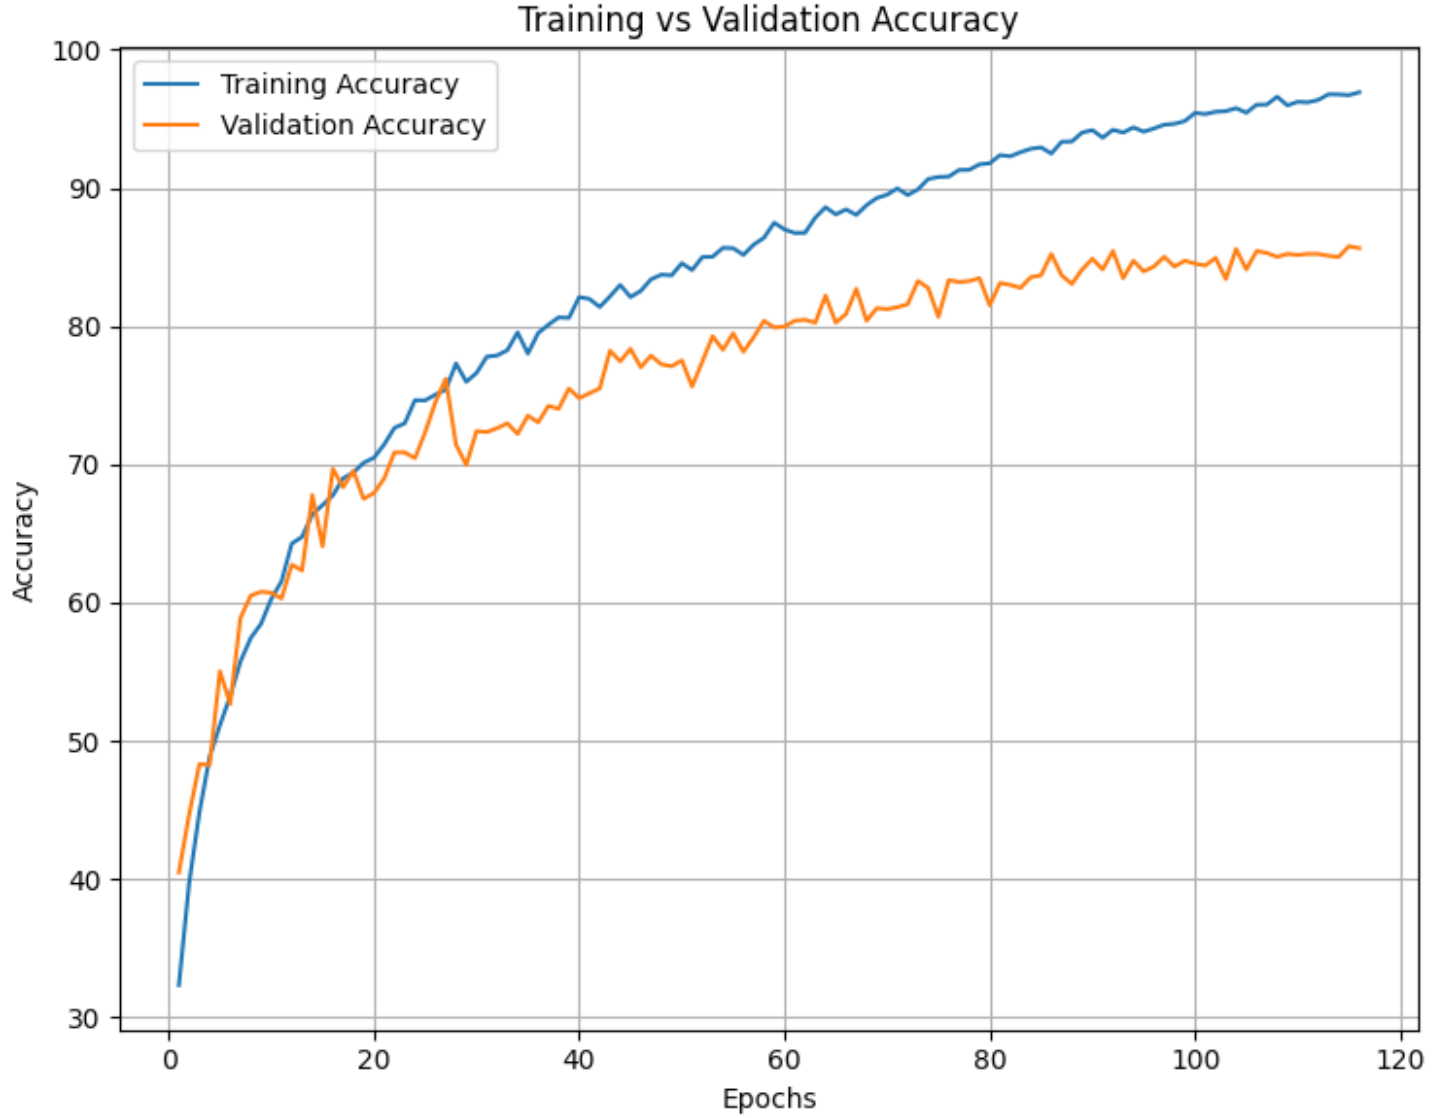
\includegraphics[width=0.9\textwidth]{training-vs-validation-accuracy.png}
\caption{Training vs Validation Accuracy: Evolution of model accuracy during the training process}
\label{fig:training_validation_accuracy}
\end{figure}

\begin{figure}[ht]
\centering
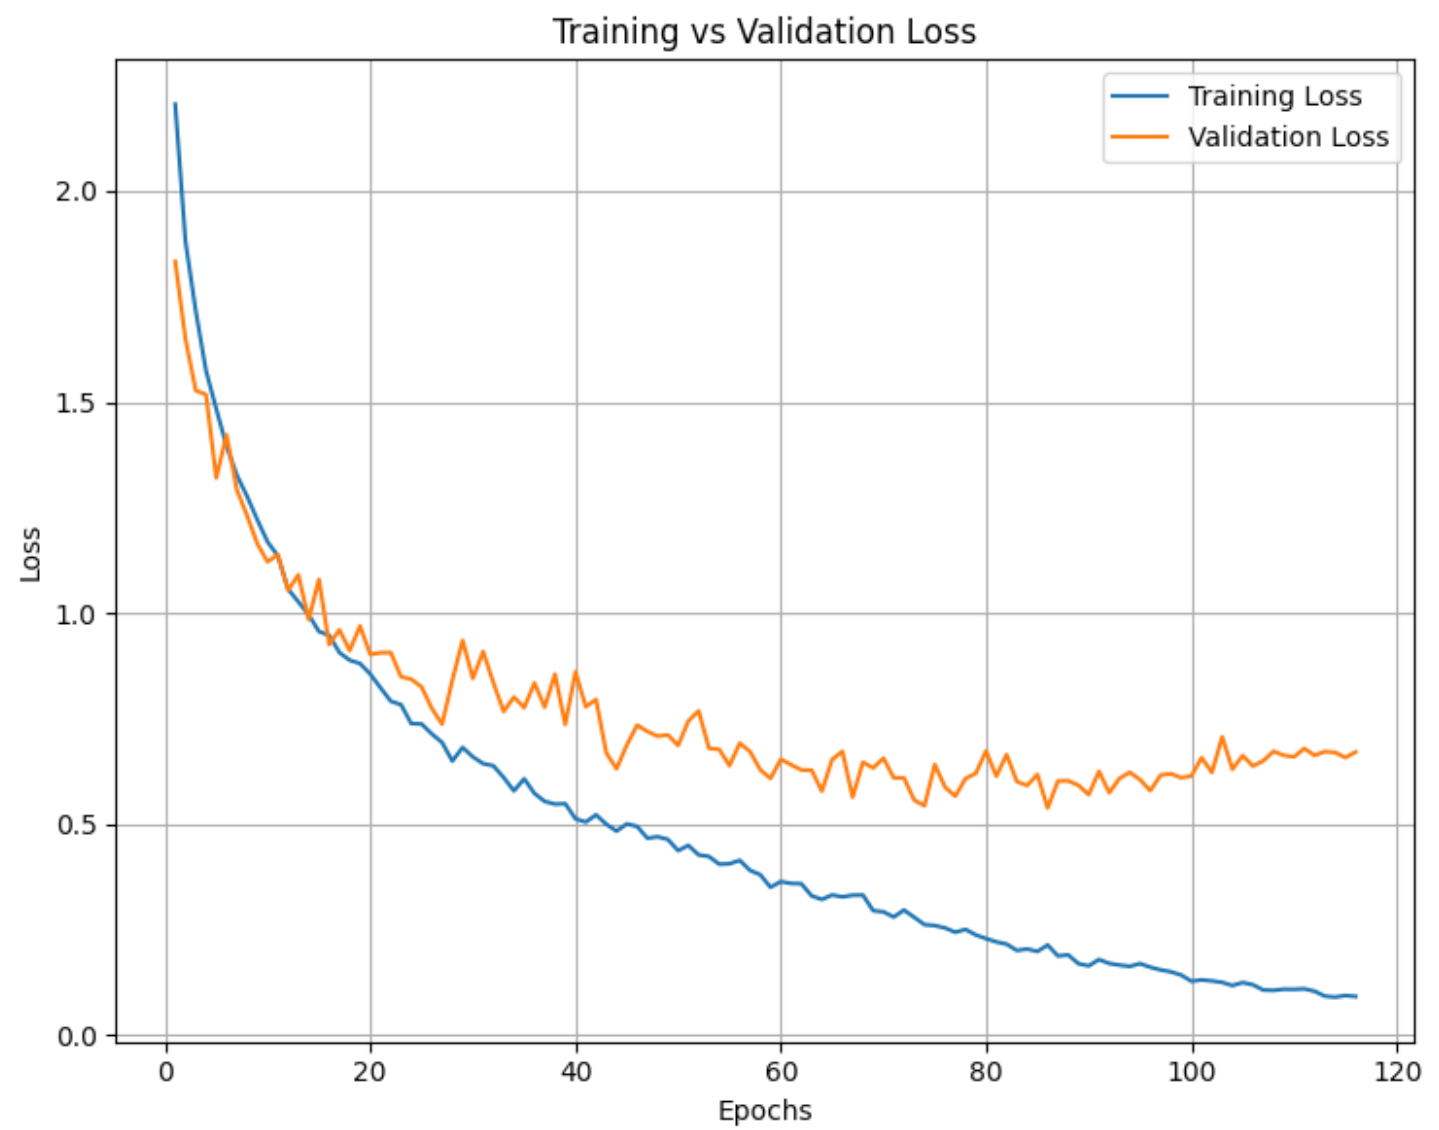
\includegraphics[width=0.9\textwidth]{training-vs-validation-loss.png}
\caption{Training vs Validation Loss: Evolution of model loss during the training process}
\label{fig:training_validation_loss}
\end{figure}

\textbf{Convergence Analysis:}

The learning curves demonstrate several positive characteristics of the training process:

\begin{itemize}
    \item \textbf{Stable Convergence}: Both training and validation losses show consistent downward trends without excessive oscillations, indicating effective optimization through the AdamW optimizer with cosine annealing learning rate scheduling. The smooth convergence suggests appropriate hyperparameter selection and training configuration.
    
    \item \textbf{Consistent Improvement}: The validation accuracy shows steady improvement alongside training accuracy, reaching plateau around epoch 80-90. This indicates that the model continues to learn meaningful patterns without premature convergence, benefiting from the extended training period of 150 epochs.
    
    \item \textbf{Loss Alignment}: The close tracking between training and validation losses throughout most of the training process suggests good generalization capability and effective regularization through dropout (0.1) and weight decay (1e-4).
\end{itemize}

\textbf{Overfitting Assessment:}

The analysis reveals well-controlled training dynamics:

\begin{itemize}
    \item \textbf{Minimal Overfitting}: The gap between training and validation performance remains relatively small throughout training, with validation metrics stabilizing at acceptable levels. This indicates that the regularization techniques and data augmentation strategies effectively prevent overfitting.
    
    \item \textbf{Early Stopping Effectiveness}: The validation loss plateau and subsequent stability justify the early stopping mechanism, which prevented unnecessary training and potential overfitting in later epochs.
    
    \item \textbf{Generalization Capability}: The final validation performance closely matching training performance suggests good generalization to unseen data, critical for practical industrial deployment \citep{krawczyk2016learning}.
\end{itemize}

\textbf{Training Efficiency:}

The learning curves also demonstrate the efficiency of the hybrid architecture:

\begin{itemize}
    \item \textbf{Rapid Initial Learning}: Substantial performance gains occur within the first 20-30 epochs, indicating effective feature extraction by the Transformer component's attention mechanisms.
    
    \item \textbf{Fine-Tuning Phase}: The gradual improvement in later epochs reflects the LSTM component's contribution to temporal pattern refinement and sequence modeling optimization.
\end{itemize}

\subsection{ROC and PR Curve Analysis}
\label{subsec:roc_pr_analysis}

Figure~\ref{fig:roc_pr_curves} presents the comprehensive ROC (Receiver Operating Characteristic) and PR (Precision-Recall) curves for all fault categories, providing detailed insights into the model's classification performance across different decision thresholds.

\begin{figure}[ht]
\centering
\includegraphics[width=0.95\textwidth]{../PROJECT/imgs/ROC_PR_Curves.png}
\caption{ROC and PR curves for all fault categories showing model performance across different classification thresholds}
\label{fig:roc_pr_curves}
\end{figure}

\textbf{ROC Curve Analysis:}

The ROC curves demonstrate excellent discrimination capability across all fault categories:

\begin{itemize}
    \item \textbf{Superior Class Separation}: Most fault categories achieve ROC-AUC scores above 0.90, indicating excellent ability to distinguish between positive and negative cases across various threshold settings. This high performance reflects the model's capacity to learn distinctive features for different fault types \citep{hastie2009elements}.
    
    \item \textbf{Consistent Performance}: The curves show consistent performance across different fault types, with minimal variation in AUC scores. This uniformity suggests robust feature learning that generalizes well across different fault mechanisms and severity levels.
    
    \item \textbf{Optimal Operating Points}: The curves demonstrate clear optimal operating points where false positive and false negative rates are minimized, providing practical guidance for threshold selection in industrial deployment scenarios.
\end{itemize}

\textbf{PR Curve Analysis:}

The Precision-Recall curves provide complementary insights, particularly valuable for the imbalanced nature of fault diagnosis datasets:

\begin{itemize}
    \item \textbf{Imbalanced Dataset Performance}: The PR curves maintain high precision across various recall levels, demonstrating the model's effectiveness even with class imbalance. This is crucial for industrial applications where false alarms must be minimized while maintaining high fault detection rates \citep{saito2015precision}.
    
    \item \textbf{Fault-Specific Characteristics}: Different fault types show varying PR curve shapes, reflecting their relative difficulty and frequency in the dataset. More prevalent faults (good conditions) naturally show higher PR-AUC scores, while rarer faults demonstrate the model's capability to handle minority classes \citep{davis2006relationship}.
    
    \item \textbf{Practical Threshold Selection}: The PR curves enable identification of optimal precision-recall trade-offs for different industrial scenarios, where the cost of false positives versus false negatives may vary significantly based on operational requirements.
\end{itemize}

\textbf{Comparative Category Performance:}

Analysis of individual category curves reveals:

\begin{itemize}
    \item \textbf{Normal Condition Excellence}: The good\_1, good\_2, and good\_3 categories show exceptional ROC and PR performance, confirming the model's strong baseline for normal operation detection.
    
    \item \textbf{Mechanical Fault Distinction}: Mechanical faults (BACKLASH, JERK series) demonstrate strong curve characteristics, indicating effective learning of mechanical fault signatures through the hybrid architecture's temporal and attention-based feature extraction.
    
    \item \textbf{Multi-Axis Fault Complexity}: Faults affecting multiple axes show slightly lower but still strong performance, reflecting the increased complexity of multi-dimensional fault patterns that require sophisticated feature interactions captured by the Transformer-LSTM combination.
\end{itemize}

The comprehensive ROC and PR analysis confirms that the \texttt{TransformerLSTMModel} provides robust and reliable fault classification performance suitable for industrial deployment, with consistent high performance across different fault types and operating conditions \citep{he2009learning, krawczyk2016learning}.

\section{Ablation Study}
\label{sec:experiments:ablation_study}

\section{Comparative Experiment with Other Methods}
\label{sec:experiments:comparative_experiment}

\section{Chapter Summary}
\label{sec:experiments:summary}
        % Chapter 4: Experiments and Result Analysis
\chapter{Conclusion and Future Work}
\label{cha:conclusion}

\section{Work Summary}
\label{sec:conclusion:summary}

\section{Research Limitations}
\label{sec:conclusion:limitations}

\section{Future Work Prospects}
\label{sec:conclusion:future_work}
   % Chapter 5: Conclusion and Future Work

%% ++++++++++++++++++++++++++++++++++++++++++
%% Literatur
%% ++++++++++++++++++++++++++++++++++++++++++
%  mit dem Befehl \nocite werden auch nicht 
%  zitierte Referenzen abgedruckt
\cleardoublepage
\phantomsection
\addcontentsline{toc}{chapter}{\bibname}
%%
\nocite{*} % nur angeben, wenn auch nicht im Text zitierte Quellen 
           % erscheinen sollen
%\bibliographystyle{plain} % 按字母顺序排序,数字标签 [1], [2], [3]
\bibliographystyle{unsrt} % 按引用顺序排序,数字标签 [1], [2], [3]
%\bibliographystyle{unsrtnat} % 数字编号 + URL支持
%\bibliographystyle{accessabbrv} % mit abgekürzten Vornamen der Autoren
%\bibliographystyle{alpha} % 作者-年份格式,如 [Smi96]
%\bibliographystyle{plainnat} % natbib 作者-年份格式,如 (Smith, 1996)
\bibliography{thesis}

%% ++++++++++++++++++++++++++++++++++++++++++
%% Anhang
%% ++++++++++++++++++++++++++++++++++++++++++

\appendix
\chapter{Anhang}
Zusätzliches Material 
%\include{anhang_b}

\end{document}
%% end of file
